\documentclass[12pt]{scrreprt}
\usepackage[english]{babel}
\usepackage[utf8]{inputenc}
\usepackage[T1]{fontenc}
\usepackage{textcomp}
\usepackage{natbib}
\usepackage{amsmath}
\usepackage{graphicx}
\usepackage{appendix}
%\usepackage[colorlinks, linkcolor=magenta, citecolor=red]{hyperref}
\usepackage[acronym, toc]{glossaries}
\usepackage{float}
\usepackage{csquotes}
\usepackage{caption}

\usepackage{listings}
\usepackage{caption}
\usepackage{minted}
\usepackage{float}
\usepackage{array}
\usepackage{tabularx}
\usepackage[table]{xcolor}
\usepackage{makecell}
\usepackage{enumitem}

% https://latexcolor.com/
\definecolor{flavescent}{rgb}{0.97, 0.91, 0.56}
\definecolor{flax}{rgb}{0.93, 0.86, 0.51}
\definecolor{paleaqua}{rgb}{0.74, 0.83, 0.9}
\definecolor{paleblue}{rgb}{0.69, 0.93, 0.93}
\definecolor{periwinkle}{rgb}{0.8, 0.8, 1.0}
\definecolor{persiangreen}{rgb}{0.0, 0.65, 0.58}
\definecolor{mediumturquoise}{rgb}{0.28, 0.82, 0.8}
\definecolor{mayablue}{rgb}{0.45, 0.76, 0.98}
\definecolor{lightskyblue}{rgb}{0.53, 0.81, 0.98}
\definecolor{magicmint}{rgb}{0.67, 0.94, 0.82}



\newcommand{\mq}{How can a real-time safety module be designed and implemented that prevents injury to patients or damage to the environment because of collision, clamping or pinching caused by care robot Rose?}
% Interface to Rose. Communication over ethernet, fast enough.
\newcommand{\sqone}{What hardware and operating system can be used to implement a safety module that has real-time constraints for care robot Rose?}
\newcommand{\sqtwo}{How can sensor and actuator data be retrieved?}
% Certain things that cannot be done mechanically (essentially why we need to use the safety module in the first place).
\newcommand{\sqthree}{How can sensor and actuator data be used to check for unsafe behaviour?}
% This should specify the entire deal having to do with the modelling real-time constraints in dezyne and the other means of verification of the safety module.
\newcommand{\sqfour}{How can the safety module be modelled in relation to the real-time care robot such that the model guarantees that unsafe behaviour is detected and signalled and that the safety module meets all of its deadlines?}
\newcommand{\sqfive}{How can we implement the model on the hardware and how can we implement it in software?}

 
\usepackage[style=apa]{biblatex}
\addbibresource{bib.bib}

 
\makeglossaries

% No indents after pars
\setlength\parindent{0pt}

\usepackage[colorlinks, linkcolor=black, citecolor=black]{hyperref}

\DeclareCiteCommand{\cite}
  {\usebibmacro{prenote}}
  {\usebibmacro{citeindex}%
   \printtext[bibhyperref]{\usebibmacro{cite}}}
  {\multicitedelim}
  {\usebibmacro{postnote}}

\DeclareCiteCommand*{\cite}
  {\usebibmacro{prenote}}
  {\usebibmacro{citeindex}%
   \printtext[bibhyperref]{\usebibmacro{citeyear}}}
  {\multicitedelim}
  {\usebibmacro{postnote}}

\DeclareCiteCommand{\parencite}[\mkbibparens]
  {\usebibmacro{prenote}}
  {\usebibmacro{citeindex}%
    \printtext[bibhyperref]{\usebibmacro{cite}}}
  {\multicitedelim}
  {\usebibmacro{postnote}}

\DeclareCiteCommand*{\parencite}[\mkbibparens]
  {\usebibmacro{prenote}}
  {\usebibmacro{citeindex}%
    \printtext[bibhyperref]{\usebibmacro{citeyear}}}
  {\multicitedelim}
  {\usebibmacro{postnote}}

\DeclareCiteCommand{\footcite}[\mkbibfootnote]
  {\usebibmacro{prenote}}
  {\usebibmacro{citeindex}%
  \printtext[bibhyperref]{ \usebibmacro{cite}}}
  {\multicitedelim}
  {\usebibmacro{postnote}}

\DeclareCiteCommand{\footcitetext}[\mkbibfootnotetext]
  {\usebibmacro{prenote}}
  {\usebibmacro{citeindex}%
   \printtext[bibhyperref]{\usebibmacro{cite}}}
  {\multicitedelim}
  {\usebibmacro{postnote}}

\DeclareCiteCommand{\textcite}
  {\boolfalse{cbx:parens}}
  {\usebibmacro{citeindex}%
   \printtext[bibhyperref]{\usebibmacro{textcite}}}
  {\ifbool{cbx:parens}
     {\bibcloseparen\global\boolfalse{cbx:parens}}
     {}%
   \multicitedelim}
  {\usebibmacro{textcite:postnote}}



\begin{document}

% Syntax highlighting for my code.
\lstdefinestyle{customc}{
  belowcaptionskip=1\baselineskip,
  breaklines=true,
  frame=L,
  xleftmargin=\parindent,
  language=C++,
  showstringspaces=false,
  basicstyle=\footnotesize\ttfamily,
  keywordstyle=\bfseries\color{blue},
  commentstyle=\itshape\color{green!40!black},
  identifierstyle=\color{violet},
  stringstyle=\color{red},
}

\lstset{escapechar=@,style=customc}


\begin{titlepage}

\newcommand{\HRule}{\rule{\linewidth}{0.5mm}} % Defines a new command for the horizontal lines, change thickness here

\center % Center everything on the page
 
%----------------------------------------------------------------------------------------
%    HEADING SECTIONS
%    HEADING SECTIONS
%----------------------------------------------------------------------------------------

\textsc{\Large Inholland University of Applied Science}\\[1.5cm] % Name of your university/college
\textsc{Bachelor Thesis in Computer Engineering}\\[0.5cm] % Major heading such as course name
%\textsc{\large Minor Heading}\\[0.5cm] % Minor heading such as course title

%----------------------------------------------------------------------------------------
%    TITLE SECTION
%----------------------------------------------------------------------------------------

\HRule \\[0.4cm]
{ \LARGE \bfseries Design and Implementation of a Real-time Safety Module for Care Robots}\\[0.4cm] % Title of your document
\HRule \\[1.5cm]
 
%----------------------------------------------------------------------------------------
%    AUTHOR SECTION
%----------------------------------------------------------------------------------------

\begin{minipage}{0.4\textwidth}
\begin{flushleft} \large
\emph{Author:}\\
Kaydo Alders % Your name
\end{flushleft}
\end{minipage}
~
\begin{minipage}{0.4\textwidth}
\begin{flushright} \large
% TODO: Add name titles
\emph{Supervisors:} \\
Cock Heemskerk \\ % Supervisor's Name
Ton Boode\\ % Supervisor's Name
Elmer Hoeksema \\ % Supervisor's Name
\end{flushright}
\end{minipage}\\[2cm]

% If you don't want a supervisor, uncomment the two lines below and remove the section above
%\Large \emph{Author:}\\
%John \textsc{Smith}\\[3cm] % Your name

%----------------------------------------------------------------------------------------
%    DATE SECTION
%----------------------------------------------------------------------------------------

{\large \today}\\[2cm] % Date, change the \today to a set date if you want to be precise

%----------------------------------------------------------------------------------------
%    LOGO SECTION
%----------------------------------------------------------------------------------------

%\includegraphics{logo.png}\\[1cm] % Include a department/university logo - this will require the graphicx package
 
%----------------------------------------------------------------------------------------

% TODO: Add Verum et al. 
\Large Research group robotics

\begin{center}
    
\includegraphics[width=0.5\textwidth]{Figures/inholland.jpg}
\end{center}

\vfill % Fill the rest of the page with whitespace
\end{titlepage}

\pagenumbering{roman}
% Also see the format from moodle.
% TODO: Look into below.
%%%
%Omslag
%    • niet verplicht
%    • Op de omslag staat alleen de titel, de naam van het bedrijf waar het onderzoek is uitgevoerd en de auteur (= naam van de student). De volledige gegevens staan op het titelblad.
%Titelblad
%
%
%
%
%
%
%
%Eerste blad na titelblad
%    • complete titel en eventueel ondertitel
%    • naam student en studentnummer
%    • datum en plaats
%    • Naam opleiding
%    • Hogeschool Inholland
%    • naam en plaats afstudeerbedrijf 
%    • naam afstudeerbegeleider
%
%    • plagiaatverklaring (zie blackboard voor een voorbeeld)
%
%Voorwoord
%(krijgt geen hoofdstuknummer)
%    • persoonlijk (gebruik de ik-vorm)
%    • bedankje
%    • niet opnemen in de inhoudsopgave
%    • kort
%
%Samenvatting
%(krijgt geen hoofdstuknummer)
%
%    • maximaal 1 pagina A4 (ongeveer 400 woorden)
%    • aanleiding en doelstelling 
%    • onderzoeksvraag en deelvragen
%    • opzet, resultaten en belangrijkste conclusies
%    • belangrijkste aanbevelingen (indien van toepassing)
%    • alleen relevante informatie
%    • kort en bondig
%    • is zelfstandig te lezen
%%%
\chapter*{Abstract}
%\chapter*{Acknowledgements}
% TODO: Summary?
\tableofcontents
\newpage
\pagenumbering{arabic}

\chapter{Introduction}
\label{Introduction}
Research group Robotics at Inholland Alkmaar conducted the assignment to improve the safety of care robots, as in the current state of affairs the care robots cannot guarantee safety. When a component of the care robot fails, like the grip arm, motion sensor or navigational equipment it can result in major consequences like damage to the robot's environment or injury of patients. Without guarantees that these consequences will not take place Rose cannot be used in practice. Research group Robotics therefore wants to develop a safety module that can be attached to a care robot and will operate as fail operational system to prevent major consequences like damage to the care robots environment or patient injury. The safety module will constantly check if the behavior of the of the care robot is safe given the situation. The safety module is a safety critical real-time system, as its actions are required to be completed in a given time for there not to be any bad consequences and to provide an extra layer of safety over any existing safety measures.

% Perhaps add some figures from care robot rose here.
\chapter{Assignment Specification}
TODO\\
O\\
D\\
O\\

\section{Goal of the assignment}
\label{Goal of the assignment}
% In de doelstelling beschrijf je wat je met je opdracht wilt bereiken. Hierin verwijs je naar de aanleiding.

The task for the computer engineering student will be to design and implement a prototype of the safety module such as is described in Chapter \ref{Introduction}. This prototype will detect situations where the care robot could behave in an unsafe manner and will signal this to its environment. We will focus on an implementation for the semi-autonomous care robot \textit{Rose}, as this is the care robot located at Innovatielab at Inholland Alkmaar. In the case of robot Rose, the prototype safety module will provide an extra layer of safety in addition to the already existing safety measures on the robot. Section \ref{Assignment specification} describes the assignment in depth. 
 The goal is achieved when the care robot, with the safety module attached, is able to identify in software when certain situations of unsafe behavior take place and is able to signal this to its enviroment.
 
\section{Assignment specification and Problem Analysis}
\label{Assignment specification}
% In dit gedeelte beschrijf je de opdracht gedetailleerd en zo concreet mogelijk. Dit is dus een grotere uitwerking van je onderzoeksvraag.

In this section an in depth elaboration of the assignment is given.
\par
The assignment is to design and implement a prototype of a safety module for care robots. The prototype of the safety module will be implemented and tested on the semi-autonomous care robot Rose. Later models of the safety module will also have to work on different care robots, semi- and fully autonomous alike. Testing on different care robots is out of the scope for this assignment, however. The exact scope of the assignment is given in Section \ref{Scope of the assignment}. The safety module should detect situations where robot Rose could behave in an unsafe manner. For this assignment unsafe behavior is given the following definition:
\begin{flushleft}
\textit{
Unsafe behavior is behavior that could result in injury to humans or damage to the environment by collision, clamping or pinching of the care robot with an object or human.
}
\end{flushleft}
The head, body and platform can collide or clamp with an object. Pinching of an object can be caused by the grip arm's gripping force or torque.  In this section, we will further elaborate how we can design and implement a prototype of the safety module. \\
 
 %%% This is problem analysis
% From this it follows that we will look at the kinetic energy of the platform, body and head to determine its impact energy if the robot were to collide with an object. Collision as a result from Rose making a turn will be taken into account by looking at the rotational energy. Pinching can be prevented by limiting Rose her grip arm strength.
 
It should be noted that Rose already has safety measures built into her system. For example, collision with a person and electric shock due to spilling of water are prevented by using the navigation path planning and making the external housing of electrical parts water resistant. The latter is a mechanical safety measure. The former is a software safety measure, but it is not a real-time safety measure due to the fact that Rose uses \acrshort{ros}. In cases such as the former the goal of the safety module is to provide a second-layer real-time safety check that operates independently from Rose to provide extra safety measures. The keyword real-time is important here, as this really is the added benefit over the regular safety measures. Throughout the report, we use the following definition of real-time: 

\begin{flushleft}
\textit{
A real-time system is a system that must react to stimuli from a controlled object within time intervals dictated by its environment. (\cite{realtime_systems}).
}
\end{flushleft}

Thus a real-time system is given limited time to react to a given stimuli. In context of the safety module the stimuli would be, for example, the acceleration sensor on Rose detecting a large increase in velocity. In such a case the safety module would create a real-time task to signal this large increase as unsafe behaviour to its environment. The time before which the safety module must have completed the task of signalling the environment task is called the \textit{deadline} of the task. (\cite{realtime_systems}). In real-time systems often the distinction is made between hard, firm and soft real-time tasks. \cite{buttazo} gives the following definitions for these: A real-time task is said to be hard if producing the results after its deadline
may cause catastrophic consequences on the system under control, it is said to be firm if producing the results after its deadline is useless for the system, but does not cause any damage and it said to be soft if producing the results after its deadline has still some utility for the system, although causing a performance degradation.
\par
% TODO: replace later 
From our earlier given definition of the unsafe behavior the safety module has to detect, namely that it should detect unsafe behavior that could result in injury to humans, it seems quite unethical to give the real-time safety module any other designation then hard real-time, as injury to patients is severely catastrophic. Indeed, we think the final safety module should be hard real-time. In this assignment, however, we are designing and implementing a prototype, and we will accept soft real-time behavior to be good enough for two reasons. The first reason is that the safety module will communicate with Rose to receive sensor data. Rose runs \acrfull{ros}, and since \acrlong{ros} is not real-time (\cite{why_is_ros_not_realtime}), we cannot achieve hard real-time behavior, as too much latency will occur by reading sensor data from Rose. This is a bottleneck, and a large part of the research is designated to accommodating for inherently non-real-time aspects of the robot-and-safety-module system like this. The second reason is that we will develop a prototype and that the development time is too small to investigate and realise the requirements for hard real-time systems.

\section{Deliverables}
\label{Deliverables}
% Deze paragraaf bevat de specificatie van de op leveren producten zoals aangegeven door de opdrachtgever.
The deliverables of this research are as follows:

\begin{itemize}
    \item A thesis containing the results of the research.
    \item A prototype implementation of the safety module.
    \item Software models of the safety module's behavior and functionality.
    \item Installation documentation of hardware and software used for the safety module
    \item Documentation of the source code, either in the respective source code files or as a separate document
\end{itemize}

\section{Involved parties}
\label{Parties involved and communication scheme}
The following table represents the parties involved in the research and their function in the research.
% Beschrijf in dit deel van je plan van aanpak welke partijen betrokken zijn bij je onderzoek. Beschrijf onder meer in welke organisatie/afdeling deze personen werkzaam zijn en wat hun functie is. Noteer hun mailadressen en telefoonnummers.
% Daarnaast vermeld je hoe de communicatie met deze personen gaat verlopen: de termijn van overleg, evt. tijdstip, de manier van communiceren et cetera.
The involved parties of this research are given in Table \ref{tab:involved-parties}. For each party, the university or company they work for, their name, their email address and their function in this research are listed.

%TODO: Perhaps add full name.
% Please add the following required packages to your document preamble:
\begin{table}[H]
{\rowcolors{1}{magicmint}{paleblue}
\resizebox{\textwidth}{!}{%
\begin{tabular}{|l|l|l|l|}
\hline
\multicolumn{1}{|r|}{\textbf{University / Company}} & \textbf{Name} & \textbf{Contact} & \textbf{Function in research}\\ \hline
Inholland & Cock Heemskerk & cock.heemskerk@inholland.nl & Supervisor company\\ \hline
Inholland & Ton Boode & ton.boode@inholland.nl & Supervisor company\\ \hline
Inholland & Elmer Hoeksema & elmer.hoeksema@inholland.nl & Supervisor university\\ \hline
Inholland & Pieter van den Hoeven & pieter.vanderhoeven@inholland.nl & Financial insights\\ \hline
TU Twente & Jan Broenink & j.f.broenink@utwente.nl & Implementation support\\ \hline
Verum & Bert de Jonge  & bert.de.jonge@verum.com  & Toolset support\\ \hline
Verum & Johri van Eerd & johri.van.eerd@verum.com & Modelling support\\ \hline
Heemskerk Innovative Technology & Dimitris Karageorgos & d.karageorgos@heemskerk-innovative.nl & Care robot support \\ \hline
DigiNova & Jeroen Wildenbeest & j.g.w.wildenbeest@heemskerk-innovative.nl & Acquaintance with mobile care robots \\ \hline
\end{tabular}%
}
}

\caption{Involved parties and their function in this research}
\label{tab:involved-parties}
\end{table}




\chapter{Problem Analysis and Research Questions}
\label{Problem Analysis and Research Questions}
TODO: Intro
%\section{Relevance of the assignment}
%\label{Relevance of the assignment}
% Beschrijf in de aanleiding waarom het bedrijf wil dat je deze opdracht gaat doen. Wat zijn bijvoorbeeld de consequenties voor het bedrijf wanneer de opdracht uitgevoerd wordt, of juist niet uitgevoerd wordt? Zo schets je de achtergrond en het belang van je opdracht voor het bedrijf.



\section{Hardware setup}
\label{Hardware setup}
%In this subquestion we will look at the hardware setup and see if the safety module can be implemented in such a way that the safety module could be attached to different care robots with little configuration. Further discussion on this can be found in Section \ref{}.

A Hardware setup that can handle the real-time constraints is required for the assignment. With real-time constraints we mean restrictions on the timing of tasks such that they meet their deadline. (\cite{real-time_constraints}). Although the prototype safety module will only be tested on the care robot Rose, eventually the safety module has to work on a variety of care robots. The hardware should therefore be extensible so that it can work with different care robots as well.
\par
The following are all the requirements for the hardware platform as they are relevant to our research:

\begin{enumerate}
    \item The hardware supports environments with real-time constraints. \label{hsOne}
    \item The hardware is able to communicate with care robot systems that run \acrlong{ros} to receive sensor data from such care robots. \label{hsTwo}
    \item The hardware has or supports the addition of a WiFi module for communication with the operator that controls the care robot. \label{hsThree}
    \item The hardware has or supports the addition of a 4G network module. \label{hsFour}
    \item The hardware has or supports the addition of an accelerometer, a gyroscope and a camera. \label{hsFive}
    \item The hardware can be attached to a care robot without impact on the operation of the care robot. \label{hsSix}
    \item The costs for the safety module do not exceed €300,- \label{hsSeven}
\end{enumerate}

Item \ref{hsOne} specifies that the hardware should support an environment with real-time constraints. In Section \ref{Assignment specification} we elaborate why this is required for the safety module.
\par
Item \ref{hsTwo} specifies that the hardware is required to communicate with care robot systems that run \acrlong{ros} to receive sensor data from. Robot Rose runs ROS, and many other care robots and mobile servant robots do too ((\cite{human-robot}), (\cite{spencer}), (\cite{delgado}), (\cite{dimitris}) to name a few), so if the safety module is extended to other care robots in the future it is very useful to support \acrshort{ros} well. 
\par
Item \ref{hsThree} specifies that the hardware should support a connection over WiFi to communicate with the operator of Rose. This is because Rose is a semi-autonomous care robot robot and receives navigation input from her operator over a WiFi network. In Item \ref{hsFour} the requirement of a 4G network module is listed. This 4G module serves as backup module for when then WiFi connection is very weak or lost. Research into an appropriate 4G module is out of the scope of this assignment and will be done in a later version of the safety module.
Item \ref{hsFive} lists the requirement that the safety module should support the addition of sensors with which it can independently from the care robot sense the environment. This should be at least an accelerometer to measure acceleration with, a gyroscope to measure angular velocity with, and a camera that allows the safety module to look around. These are required for two reasons. The first reason is to have independent sensors on the safety module so that the safety module does not depend on the correct operation of the sensors of the care robot, and the second reason is that there may be a lot of latency in receiving sensor data as it received from \acrshort{ros}. The camera need not be used in this assignment, but the safety module should support the addition of a camera for future versions. 
Item \ref{hsSix} refers to the fact that the safety module should be portable, that is, it easy to attach to a care robot. It should not have an impact on the performance of the care robot. This means it should be light (relative to the care robot) and should not have large components sticking out (also relative to the rest of the care robot).
Lastly Item \ref{hsSeven} specifies the maximum costs of the safety module.


is assignment, however, we are designing and implementing a prototype, and we will accept soft real-time behavior to be good enough for two reasons. The first reason is that the safety module will communicate with Rose to receive sensor data. Rose runs \acrfull{ros}, and since \acrlong{ros} is not real-time (\cite{why_is_ros_not_realtime}), we cannot achieve hard real-time behavior, as too much latency will occur by reading sensor data from Rose. This is a bottleneck, and a large part of the research is designated to accommodating for inherently non-real-time aspects of the robot-and-safety-module system like this. The second reason is that we will develop a prototype and that the development time is too small to investigate and realise the requirements for hard real-time systems.
\\
Section \ref{tHardware} shows the literature review we did to see what others have used as hardware setup for their robots.



\section{Operating system of the safety module}
As a hardware setup to handle the real-time constraints of the safety module is required, likewise a software setup that can handle the real-time constraints is required. This mainly concerns the operating system the safety module will run on. Research will be conducted to use an operating system on the safety module that can handle these constraints. In Section \ref{tOS} we elaborate the literature review we did on various qualifying operating systems.


\section{Retrieving sensor data from Rose}
\label{Retrieving sensor data from Rose}
Rose runs a Linux distribution with Robot Operating System (ROS) as middleware. To retrieve data from Rose her sensors we have to look into the available means of communication with this system. ROS is not real-time (\cite{why_is_ros_not_realtime}), therefore it is important to research the impact this has on the safety module and whether communication over the available interfaces is fast enough for a system with real-time constraints. It could be that the available interface is too slow for real-time communication. Such a case is a risk and will be elaborated in Section \ref{Risks and solutions}. The obtained sensor data will be compared with a set of \textit{limit} values in a control loop.

%These limit values are obtained by means of an external plugin that specify limitations actions the care robot is allowed to take in a given situation. The use of an external plugin will be further explained in Section \ref{Definition of unsafe behavior as a external plugin}.

%\subsection{Definition of unsafe behavior as an external plugin}
%\label{Definition of unsafe behavior as a external plugin}
%% Describe how the safety will be imported as a plug in.
%As described in Section \ref{Principal research question and research subquestions} the definition of unsafe behavior for a care robot will be obtained externally. This is because definitions for safe and unsafe behavior are situation dependent and differ per care robot. Although the initial implementation of the safety module will be tested on the care robot Rose, the safety module will have to work with different care robots in the future as well. We could define unsafe behavior for the care robot Rose, but we would then also have to determine what unsafe behavior is for different care robots with different maximum speeds, different grip strength, different platforms, etc. It is for this reason that the assignment does specify to think about the definition of safe and unsafe behavior and instead specifies that the safety module should be able to integrate a definition of unsafe behavior provided by someone else. Concretely this means that someone, for example the company that produces the care robot, provides a plugin or file containing several lists of values that should specify in what circumstances the safety module should alarm. Such a list of values is a list of \textit{limit} values, specifying for example the maximum linear and rotation speed a care robot can have in a given situation, the maximum grip strength the arm is allowed to have when the care robot is near a patient or a combination of these. These are just examples, and it is the companies task to correctly define safe and unsafe behavior in a given task. The safety module will obtain this definition as a plugin and will check whether any of the unsafe situations occur in its control loop. Taking the previous example, the control loop would check whether the speed or grip strength goes over the maximum limit in a situation. And if it does, the safety module will signal this. How the safety module will signal unsafe behavior is explained in Section \ref{Signalling unsafe behavior}.
 
%\subsection{Signalling unsafe behavior}
%\label{Signalling unsafe behavior}
%For the implementation of a prototype of the safety module, which is the goal of this assignment, signalling unsafe behavior will be kept simple. The safety module will signal unsafe behavior by blinking a LED and, in the case of a semi-autonomous care robot like Rose, send a signal to the operator at distance. We will, however, think about the set of actions the safety module

\section{Modelling the safety module}
\label{Modelling the safety module}
% Describe things concerning research into toolset to use (Dezyne) to validate deadlines are met.
% Describe further the modelling because we do not want to model the entire robot but only what is relevant for us.
In a software model the safety module and its relation to the care robot should be modelled. It is preferable to do as much verification on the state of the safety module and its actions as possible. Such a verification encompasses going through all the states of the sytem and verifying no deadlocks and livelocks occur.
The interactions of the safety module with the care robot needs to be modelled in such a way that the real-time constraints of the system can be tested and validated. This means that the model should be able to validate that tasks meet their deadlines.
% A partner of Research Group Robotics, namely the company Verum, offers a toolset to model such a real-time system \cite{verum}. In the assignment, we will make use of this toolset.
\par

 % Assignment specification?
% In Section \ref{Relevance of the assignment} it was mentioned that the care robot is a kind of safety critical real-time system. This implies that the care robots actions have deadlines and that the safety module, being a part of the care robot, will have to take into this account these deadlines and will have deadlines of itself. It is therefore required that in the design


\section{Principal research question and research subquestions}
\label{Principal research question and research subquestions}
% De onderzoeksvraag is het hart van het onderzoek. In één zin geef je aan wat je opdracht inhoudt. 
% In de regel verdeel je de onderzoeksvraag vervolgens in drie tot vijf deelvragen.
Having made our problem analysis we can setup our principal research question and research subquestions. To fulfill the goal of the assignment described in Section \ref{Goal of the assignment} and Section \ref{Assignment specification}, the following question will be central to the research and will serve as the principal research question:

\begin{flushleft}
\textit{\mq}
\end{flushleft}

To answer the principal research question four subquestions are set up. The first subquestion deals with the hardware and operating system that can be used in an implementation for the safety module of a care robot. Because the safety module is a safety critical real-time system, we need hardware and an operating system that can handle the real-time constraints of the care robot. The goal of the first subquestion is to provide an answer to this:

\begin{flushleft}
1. \textit{\sqone}
\end{flushleft}

%As This mainly concerns the capabilities of the operating system and whether the scheduler of the operating system can schedule tasks in such a way that deadlines will not be missed. Subquestion five is as follows:
%
%\begin{flushleft}
%2. \textit{\sqfive}
%\end{flushleft}

Having determined our hardware setup and operating system, we can look at ways to communicate with care robot Rose and the sensors available on our hardware. Concretely, we will look at how sensor and actuator data can be retrieved, and how it can be used to detect unsafe situations. Therefore, the second subquestion is as follows:

\begin{flushleft}
2. \textit{\sqtwo}
\end{flushleft}

% TODO: real-time -/-> deadlock handling.
After subquestion two we can start designing the safety module with a software model. In the software model we want to do as much verification on the state of the safety module and its actions as possible. Moreover, we have to take into account that the safety module will be a safety critical real-time system, as described in Section \ref{Relevance of the assignment}.
We therefore have to concern ourselves with the real-time constraints while modelling the safety module. real-time constraints encompass matters like avoiding deadlocks and meeting deadlines of tasks. The third subquestion is as follows:

\begin{flushleft}
3. \textit{\sqthree}
\end{flushleft}

The fifth and final subquestion will bring everything together into an implementation of the safety module. Here we will implement the safety module on the chosen hardware and operating system and according to the model of the previous subquestion. The last subquestion is as follows:

\begin{flushleft}
4. \textit{\sqfour}
\end{flushleft}

%%%%%%%%%%%%%%%%%%%%%%%%%%%%%% SCOPE OF THE ASSIGNMENT %%%%%%%%%%%%%%%%%%%%%%%%%%%%%%
%\section{Scope of the assignment}
%\label{Scope of the assignment}
%% Studenten zijn vaak geneigd om een veel te grote opdracht te accepteren. Het is zaak om bij het plan van aanpak al prioriteiten te stellen: wat ga je beslist doen, wat ga je zeker niet doen, en wat ga je doen als er nog tijd over is? Feitelijk prioriteer je de mogelijke invulling van je opdracht. Op deze wijze zorg je ervoor dat de verwachtingen bij de opdrachtgever, bij de school en bij jezelf niet te hoog gespannen zijn en je aan een realistische en bereikbare opdracht begint.
%
%% Ook vermeld je in dit gedeelte de randvoorwaarden die nodig zijn om je opdracht tot een succes te maken en de eisen die de opdrachtgever zelf stelt aan je opdracht. Zo maak je deze expliciet bespreekbaar voor opdrachtgever en school.
%
%
%% TODO: Use moscow here!
%% Describe how we are not concerned with what safety is, nor are we concerned with what the care robot should do in case of some detected unsafe behavior.
%
%In this chapter the scope of the assignment is provided. The scope is provided in the form of a \textit{moscow} list \cite{moscow}, specifying what \textit{must} be done to succeed the assignment, what \textit{should} be persued but does not decide success of the project, what \textit{could} be done if ti and what we \textit{would} like to have but will not be delivered this time. In Section \ref{MoSCoW list} the moscow list is shown.
%
%\subsection{Moscow list}
%\label{MoSCoW list}
%\begin{description}
%\item Must
%    \begin{itemize}
%        \item Safety module guarantees that in software eliminateable situations of collision, clamping and pinching that could result in injury of the patient or damage to the enviroment do not take place. 
%        \item Safety module lights a LED when Rose shows unsafe behavior.
%        \item Safety module is able to retrieve sensor and actuator data from Rose.
%        \item Safety module checks for unsafe behavior by comparing retrieved sensor data with data that defines unsafe behavior from a test plugin.
%        \item The software model for the safety module verifies correct real-time behavior of the safety module.
%        \item The actions of the safety module are soft real-time.
%    \end{itemize}
%\item Should
%    \begin{itemize}
%        \item Safety module signals the operator when Rose shows unsafe behavior.
%        \item The actions of the safety module are hard real-time.
%        \item Hardware setup of the safety module is generic enough to work on a variety of care robots.
%        \item Software setup of the safety module is generic enough to work on a variety of care robots.
%    \end{itemize}
%\item Could
%    \begin{itemize}
%        \item Safety module is able to restore Rose when a component fails.
%        \item Safety module is able to integrate unsafe behavior specified with multiple different plugins.
%    \end{itemize}
%\item Would
%    \begin{itemize}
%        \item Safety module minimises risk of damage or injury on a variety of care robots.
%        \item Safety module is able to control Rose's or a different care robot's wheel motors to autonomously drive the robot out of an unsafe situation.
%        \item Safety module is able to control Rose's or a different care robot's gripping arm motors to autonomously adjust force or torque in an unsafe situation.
%    \end{itemize}
%\end{description}


%\subsection{Elaboration on MoSCoW list}
%\label{Elaboration on MoSCoW list}

%%%%%%%%%%%%%%%%%%%%%%%%%%%%%% COMPETENCES %%%%%%%%%%%%%%%%%%%%%%%%%%%%%%
%\section{Competences}
%\label{Competences}
%% In deze paragraaf beschrijf je de competenties/indicatoren waaraan je door middel van je onderzoek werkt. Denk eraan dat je hierin zowel de beroepscompetenties als de competenties professionalisering en onderzoeken (zie competentiekaart op Moodle) opneemt. In het plan van aanpak neem je in ieder geval twee beroepscompetenties op niveau 3 op. Hierbij is het van belang goed na te denken over je keuze en deze ook goed te motiveren.
%In this section the chosen competences are elaborated. \\
%A list of competences is published on moodle from which a selection can be chosen. The competences are given in Dutch as they are published in Dutch. The chosen competences are cited here: 
%
%\begin{description}
%
%\item \textbf{Competentie Onderzoeken}:\\
%\textit{Niveau 3 Startbekwaam}\\
%De student toont de competentie op dit niveau aan door kennis en vaardigheden geïntegreerd toe te passen in nieuwe of onbekende omstandigheden binnen een multidisciplinaire context die breed gerelateerd is aan het vakgebied en lost complexe vraagstukken zelfstandig en op een oorspronkelijke manier op.
%
%\item \textbf{Competentie Professionaliseren}:\\
%\textit{Niveau 3 startbekwaam}\\
%De student toont de competentie op dit niveau aan door kennis en vaardigheden geïntegreerd toe te passen in nieuwe of onbekende omstandigheden binnen een multidisciplinaire context die breed gerelateerd is aan het vakgebied en lost complexe vraagstukken zelfstandig en op een oorspronkelijke manier op.
%De student verdiept alle bij niveau 1 en 2 genoemde indicatoren op het niveau ‘startbekwaam’ binnen de genoemde context.
%
%\item \textbf{Competentie Ontwerpen}:\\
%C3.1 Opstellen van een ontwerp voor een real-time \& embedded softwaresysteem met gebruik van software-architecturen
%
%\item \textbf{Competentie Realisatie}:\\
%C3.1 Bouwen, testen en beschikbaar stellen van software met behulp van een ontwikkelomgeving en daarbij gebruikmaken van bestaande software frameworks die aansluiten bij bestaande software.
%\end{description}
%
%The competence \textit{onderzoeken} is relevant to conduct a proper research for this assignment. To elaborate, the relevant aspects of the care robot have to be sorted out, as conducting research in the entire workings of the care robot would take too much time. Moreover, to conduct a proper research good research question have to be set up, which is part of this competence as well.\\
%The competence \textit{professionaleren} is about the execution of the research. This competence is relevant because it is important conduct the research in a professional way that leads to the expected result.\\
%The design of a safety module is a central aspect of the safety module and thus the competence \textit{ontwerpen} is relevant for the assignment.\\
%Lastly the competence \textit{realisatie} is relevant for the assignment because of the other central aspect of the research, namely, implementing the safety module.

%%%%%%%%%%%%%%%%%%%%%%%%%%%%%% RISKS AND SOLUTIONS %%%%%%%%%%%%%%%%%%%%%%%%%%%%%%
% Describe what to do if we cannot realise verification on software level.
%\section{Risks and solutions}
%\label{Risks and solutions}
%% Het is goed om in het beginstadium van je onderzoek na te denken over welke risico’s er kunnen opdoemen. Daarbij gaat het natuurlijk om de risico’s die specifiek betrekking hebben op jouw onderzoek en niet zozeer om algemeen geldende risico’s. Voor deze specifieke risico’s bedenk je bovendien alvast een oplossingsrichting. Deze paragraaf zorgt er met name voor dat je tijdens de uitvoering van je onderzoek alert blijft op signalen die erop wijzen dat de door jou voorziene risico’s ook realiteit worden, zodat je al in een beginstadium actie kunt ondernemen.
%
%% TODO:
%% For the risk think about the fact that it may be really hard to make the safety module work on multiple (care) robots (genericness). I also excluded it from the primarly goal described in Section 2.
%% Risk: It could be, for example, that the communication interface with Rose is too slow for real-time communication with the safety module. In this case we would have to look for an alternative way to communicate with the sensors (if this is possible at all) or decide that the safety module 
%
%In this section, potential risks specific to the assignment and potential solutions for these risks are elaborated.
%
%\begin{description}
%\item 1. It is possible that communication with ROS over ethernet is too slow for the real-time safety module.\\
%    The safety module will send commands to ROS over ethernet to retrieve signal and actuator data from care robot Rose. It is possible that this communication is too slow, as the safety module has to respond promptly to stimulus from the enviroment of Rose. In such a case we would have to look for alternatives ways to receive sensor and actuator data from Rose. One such way is to connect create an interface that directly connects to Rose without the need of an middleware like ROS. This however would complicate a few things since all of the sensor data that is presented by Rose is stored in a ROS object.
%\item 2. It is possible that the safety module is not generic enough to work with care robots beside Rose.\\
%    ROS is not the bottleneck here since different care robots running ROS should still provide their sensor data using the same data object. However, it could be the case that the software written for the safety module interprets the data in such a way that it is dependent on what care robot it operates for. This can be avoided by taking into account from the beginning that the safety module will eventually have to work with care robots beside Rose and create the software without hardcoded values that depend on specific parts of Rose.
%\end{description}


%%%%%%%%%%%%%%%%%%%%%%%% APPROACH %%%%%%%%%%%%%%%%%%%%%%%%
%\section{Approach}
%\label{Approach}
%% In het hoofdstuk Aanpak beschrijf je hoe je denkt te werk te gaan met je opdracht. Hier wordt de brug geslagen tussen het afgebakende resultaat en de inrichting van het onderzoek, door middel van beantwoording van de hoe-vraag.
%% Beschrijf waar je mee bezig bent, kijk welke relevante theorieën beschikbaar zijn en pas deze toe bij het uitvoeren van je opdracht. Met andere woorden: zoek uit wat er vanuit de theorie al bekend is over je onderwerp en koppel hieraan je uitgangspunten, onderzoeksvraag en deelvragen. Zo onderbouw je het geheel met relevante vakliteratuur.
%
%% Stap voor stap beschrijf je de activiteiten die je denkt te moeten uitvoeren om tot het gewenste resultaat te komen. Natuurlijk zul je dit voor de korte termijn veel gedetailleerder kunnen beschrijven dan voor de wat langere termijn. Het is dan ook niet erg dat je de wat later uit te voeren activiteiten globaler beschrijft. 
%
%The approach used to provide an answer to the principal research question: \textit{\mq}, will be described in this section.\\
%First research has to be conducted into creating a hardware and software setup for the safety module. It is important that the hardware and software is able to handle the safety module's real-time constraints. Various real-time hardware options exist, a popular option is the use of microcontrollers because they do not run a operating system and thus have no overhead in scheduling user processes (\cite{realtime_scheduling}). Software will be chosen based on the hardware. A visit will be made to project partner Heemskerk Innovative Technology (\cite{hit}) to see what kind of hardware and software robot Rose already uses. This is relevant for the safety module because the hardware and software for the safety module can then also be chosen based on the existing hardware and software on the care robot.
%\\\\
%After choosing an appropriate hardware and software setup research can be conducted into communication from the safety module with robot Rose. From the assignment specification in Section \ref{Assignment specification} we know that Rose runs a Linux distribution with Robot Operating System (ROS) as middleware. We therefore want to look into the way ROS provides data from sensors and actuators so that it can be retrieved by the safety module. \cite{gentle} should provide use with enough information on how to interface with ROS.
%\\\\
%\cite{tadele} shows how previous studies implemented checks on safety for care robots. We will look into a method that is relevant to us.
%\\\\
%We will look into a method to model the behavior of the safety module in relation to the care robot. Project partner Verum developes a toolset for verification of program behavior, generation of models and generation of source code. A visit will be made to the company to see if the toolset can be used for the development of the safety module. If the toolset is useful, we can examine its documentation (\cite{verum}).
%\\\\
%The studies shown by \cite{tadele} can also be examined on how to create an implementation of the safety module from the model.

%%%%%%%%%%%%%%%%%%%%%%%% Research Methodology %%%%%%%%%%%%%%%%%%%%%%%%
\chapter{Research Methodology}
%    • per deelvraag uitwerken
%    • welke methoden zijn er gebruikt om informatie te verzamelen? Hoe ziet deze eruit? Waarom gekozen voor deze methode? Geef een toelichting. 
%    • bij interviewen: welke mensen (functies) heb je geselecteerd? Waarom?
%    • geef aan hoe je ervoor hebt gezorgd dat de informatie betrouwbaar  en valide is.
%    • geef aan hoe je de informatie hebt geanalyseerd.
%\chapter{Practical and Theoretical Background}

\section{General methodology of the research}
The general methodology of this research is a feasibility study; in the sense that we want to explore existing research in robotic control systems, real-time systems that deal with inherently non-real-time elements, verification of system behavior and mobile robotic safety. The goal is to apply these existing ideas to our case with care robot Rose, namely to implement a prototype safety module to show the feasibility of applying these ideas to the case of care robot Rose. Because of this broad focus we only touch the surface of the vast sea of knowledge that is contained in each of these subjects. To elaborate, in the context of real-time systems we will not aim for hard real-time performance of the safety module, despite care robot Rose being perceived as a hard real-time system, as this requires much more specialised attention to implement, which would deviate from our aim to explore a multitude of ideas. Instead, we aim for the safety module to be a soft real-time system that is able to show the feasibility of the system as a whole. In the context of robot safety, we will look at the safety criteria and safety measures in existing research, but in our case we will only use a rudimentary form of these safety measures criteria. Likewise we explore the ideas of system behavior verification in so far this gives guarantees on the correct operation of the safety module.
\\\\
% TODO: ref recommendations
The results of this research and the prototype safety module produced by this research can be used to built further upon the ideas explored. Specifically, this research can be used to continue the development of the safety module into a product that provides an extra layer of safety to different care robots and perhaps different mobile service robots as a whole. Chapter \ref{} elaborates follow-up research options in more depth. 
\\\\
To provide answers to the subquestions stated in Chapter \ref{Problem Analysis and Research Questions}, a mixture of research methods are used. These are elaborated per subquestion in Section \ref{Methodologies per subquestion}.

\section{Methodologies per subquestion}
\label{Methodologies per subquestion}
The first subquestion stated in Chapter \ref{Problem Analysis and Research Questions} is: '\sqone'. For this subquestion we will conduct a literature review to determine what kind of hardware previous researches use in their robotic applications. Concretely, we would like to to find hardware that is both able to handle the real-time constraints of the care robot and that can interact with \acrshort{ros}. A comparative study will be conducted to determine what is the best choice for the heart of the system, the processing unit, RAM and related peripherals. From here on we will determine what measuring devices can be used with this hardware, and we will conduct another literature review and comparative study to find an appreciate real-time operating system for this hardware of the safety module. The literature review on the hardware and software can be found in Section \ref{tHardware} and Section \ref{tOS} respectively. The results of the comparative studies can be found in the results chapter in Section \ref{Main component} and Section \ref{Operating System} respectively.
\\\\
% TODO: ref to section containing these results.
The second subquestion, '\sqtwo', builds upon the results of the first subquestion and uses the results of the comparative studies of the first subquestion to find out how, with the chosen hardware and software, we can interact with sensors to retrieve data and how we can use that data to detect unsafe behavior.
\\\\
% TODO: ref to section containing these results.
The third subquestion, '\sqthree', aims to model the behavioral aspects of the safety module. The result of this subquestion will be a formal model that can put some guarantees on the behavior of the safety module. An elaboration of the toolset that will be used to make this formal model is give in Section \ref{Modelling and Dezyne}. The results of this subquestion can be found in Section \ref{}.
\\\\
The fourth and last subquestion, '\sqfour' will put everything together in an implementation of the formal model on hardware and software. A simulation will be used to emulate the interaction with care robot Rose her sensors.


\chapter{Theoretical Background and Literature Review}
% TODO: Edit introduction when more literature review is added.
In this chapter we provide the theoretical background and literature reviews that corroborate our research. We will first present definitions of terms that are used throughout this research. After that, we present our conducted literature reviews on the topics of hardware and operating systems of service robots.
\label{Theoretical Background}
%\section{Practical background}
%     • waar speelt het onderzoek zich af (branche, bedrijf, afdeling)

%\section{Theoretical background}
%    • begripsafbakening (wat versta je onder de begrippen die een rol spelen bij het onderzoek? Vaak gaat het om de begrippen in de onderzoeksvraag.)
%    • eventueel eerder onderzoek 
\section{General terms and definitions}
\label{Terms and defintions}
Throughout the research we make use of a variety of terms and definitions. The definitions we use for \textit{real-time systems} and \textit{hard, firm and soft} real-time tasks were given in Section \ref{Assignment specification}. Likewise, the definition we use for \textit{unsafe behavior} was given in in Section \ref{Assignment specification} as well. In Section \ref{Safety in care robots} we elaborate more on the safety measures used in care robots.
\\\\
Previous research frequently uses the terms \textit{mobile service robot}, \textit{domestic robot}, personal care-robot for mobile robots used in medical (\cite{medical}) and military (\cite{military}), or for use in personal care (\cite{personal}). \citeauthor{tadele} defines a personal care-robot as a service robot with the purpose of either aiding or performing actions that contribute toward the improvement of the quality of life an individual. \citeauthor{tadele} defines a domestic care robot as a personal-care robot with or without manipulators that operate in home environments and is often mobile. When we refer to \textit{care robots} in our research, we refer to the definition of a domestic care robot as given by \citeauthor{tadele}. We sometimes refer to service robot as well, if that is the specific term used by in research we refer to.
\\\\
Multiple times in this research we refer to the concepts of \textit{processes} and \textit{threads}. A process is a sequence of execution in a computer, it is a program in execution. A process has its own address space and system resources (\cite{process_threads}). A thread is also a sequence of execution, but a thread can be seen as a subset of a process. A process can create multiple threads and each threads shares their address space and system resources with each other. (\cite{process_threads}). We sometimes use the term \textit{task} as a synonym for thread in this research.
\par
Two concepts related to processes and threads are the concepts of \textit{deadlock} and \textit{livelock}. Deadlock occurs in a system when all its constituent processes are blocked. Another way of saying this is that the system is deadlocked because there are no eligible actions that it can perform (\cite{ltsa}). One example of a deadlock in a system is a system in which two threads each hold a resource that the others requires to continue execution. Livelock occurs in a system where a thread's further execution requires the action of another executing thread, but the other thread is constantly served more work to do without executing the required action, meaning the first thread cannot continue to execute (\cite{livelock_starvation}).
\par
Two other concepts related to the execution of threads are the concepts of \textit{starvation} and \textit{race-conditions}. Starvation describes a situation where a thread is unable to gain regular access to shared resources and is unable to make progress (\cite{livelock_starvation}). A race condition occurs when two threads access a shared variable at the same time (\cite{race_condition}). Race conditions can be prevented by use of mutexes or semaphores. A mutex is a lockable object that is designed to signal when critical sections of code need exclusive access, preventing other threads with the same protection from executing concurrently and access the same memory locations \cite{mutex}. Such a critical section can be a shared variable as with a race condition. A semaphore object is a synchronization object that maintains a count between zero and a specified maximum value (\cite{semaphore}). Both mutexes and semaphores can be used to prevent race conditions.
\\\\
Definitions and meanings for terms and acronyms like, \textit{\acrshort{ros}}, \textit{\acrshort{mcu}} and \textit{\acrshort{pi}} are given in our Glossary and Acronyms lists which can be accessed by clicking on the respective term or acronym.
\par
Other definitions of terms will be given as we meet them.
    

% TODO: Some more text?
\section{Robot Operating System}
\label{tROS}
Care robot Rose uses \acrfull{ros} as its middleware. The definition of \acrfull{ros}, as given by ROS \cite{ros_wiki_introducton} is as follows:
\textit{ROS is an open-source, meta-operating system for your robot. It provides the services you would expect from an operating system, including hardware abstraction, low-level device control, implementation of commonly-used func tionality, message-passing between processes, and package management. It also provides tools and libraries for obtaining, building, writing, and running code across multiple computers.}\\
 The advantages of ROS over other robotics platforms are its distributed computation model, the ability to reuse software and the rapid testing of software build with ROS. (\cite{agitr}).
 
 \section{Safety measures used for care robots}
 \label{Safety in care robots}
There are three widely used measures for safety in care robots. These are: acceleration-based criteria,  force-based criteria and energy/power-based criteria. Other criteria include human pain tolerance, maximum stress and energy density (\cite{tadele}). Of the acceleration-based criteria, the head injury criteria (HIC) is most widely used. It is a measure of the head acceleration for an impact that lasts for a certain duration (\cite{hic}). Force-based criteria consider excessive force as the possible cause of collision injury (\cite{force}). Lastly energy/power based criteria is a criteria that considers the rate of transfer of kinetic energy on body impact as the cause of possible injury to a human (\cite{crucial_milestone}).
\par
The prototype safety module will use a very rudimentary form of force-based and energy-based safety criteria. It will calculate the kinetic energy of the body of the care robot and force used by the grip arm of the care robot and will use this as the basis to determine what is unsafe behavior. The reason we only use this rudimentary form is because research into the topics of the various safety criteria is not the focus of this research. Instead, the focus of this research is to provide second-layer real-time safety checks on care robot Rose, that are not dependent on the state of Rose her own system. We describe the goal and specification of the assignment more in depth in Section \ref{Goal of the assignment} and Section \ref{Assignment specification} respectively.
 

\section{Hardware in service robots}
\label{tHardware}
Previous research has used a variety of hardware for their real-time mobile service robot applications. \citeauthor{delgado} used a Raspberry Pi 3 as their control architecture for its open source enviroment They mention its advantages over (also open-source) embedded hardware. Developing a real-time enviroment on embedded hardware is complex due to its limited availability of systematic documentation and technical support. Although manufacturers often provide linux kernel sources, many times the system lacks compatibility with other software, which is an open problem in embedded development in general. \citeauthor{delgado} further notes that the \gls{pi} 3 offers great compatibility with \acrfull{ros}, as \acrshort{ros} offers pre-built binaries for Ubuntu systems, and the \gls{pi} 3 is able to run Ubuntu. \acrshort{ros} supports Raspbian, the native operating system of the \gls{pi} as well, but there are no pre-built  binaries for this system, which increases development time.
\par
\citeauthor{bouchier} researched into ways to integrate \acrshort{ros} into a robot. His research applied to a broader field of robots than only care robots, but his research is relevant nonetheless. He mentions three architecture styles, namely embedding \acrshort{ros} on an integrated personal computer, the use of a proprietary embedded system with custom interface and the extension of \acrshort{ros} messaging and APIs. The embedded PC architecture style allows for full integration of \acrshort{ros} on a Linux distribution with the ability to run others \acrshort{ros} nodes besides the robot system as well. Still, default Linux is not real-time, and requires patches and frameworks like Xenomai to achieve soft or firm real-time performance. For the second option, the use of a custom proprietary embedded system, \citeauthor{bouchier} describes a ROS device node can be setup to allow translation between ROS nodes and the propriety embedded interface. A recent development of the time has setup such an architecture on an Arduino (\cite{bouchier}). \citeauthor{arduino} also use an Arduino board in their wireless sensor network control system for environmental sensing of temperature and humidity. The third architecture  option describes communication with ROS nodes by use of Remote Procedure Calls (RPC). Rosserial is an approach that can be used to relay messages between ROS nodes to a embeddded system. Rosserial offers support for any platform that supports the C++ programming language.
\par
The architecture styles that \citeauthor{bouchier} describes are focused on the control system of a robot itself. In our case, the safety module is an addition to the already existing care robot system. The system of robot Rose most closely resembled the first architecture \citeauthor{bouchier} describes, but without real-time patches or a real-time framework installed. \citeauthor{bouchier}'s research is relevant nonetheless to see what kind of architecture options exist.
\par
Another architecture not described by \citeauthor{bouchier} but which can be found in, for example, (\cite{spencer}) is the use of a base CPU in the robot itself, which communicates with another PC to receive input to determine which actions to take. \citeauthor{spencer} used this in a service robot that guides and informs passengers in airports. Robot Rose has a similar architecture in that she receives navigational commands from the operator connected to her via a laptop on the WiFi network. 
\par
Instead of a PC one could also use a Field Programmable Gate Array (FPGA) as main processing unit in a service robot, as \citeauthor{visual_xenomai} has done in their patrol service robot, in which the FPGA is used for image processing to decide a travel route for the patrol robot. 
\par
Lastly, microcontrollers are also used in robotic control applications (\cite{microcontroller1}) (\cite{microcontroller2}). An advantage of using a microcontroller for the safety module would be that it does not add yet another PC with operating system to the system (Rose already has \texttt{rosepc1} and \texttt{rosepc2} which are PCs running Linux distributions) and a microcontroller is lower on power.

\section{Operating systems on service robots}
\label{tOS}

Service robots often run Linux distributions. As \citeauthor{delgado} describes, this is due to the fact that Linux operating system are the most popular open-source operating systems, and due to the development of real-time extensions for the Linux kernel to increase its response time and make it more suitable for real-time applications. Another reason Linux operating systems are popular is because \acrshort{ros} runs on Linux. In Section \ref{tHardware} we have seen that \cite{spencer} and \cite{delgado} use \acrshort{ros} as middleware on their service robots, and others do too, for example \cite{dimitris} in their Human aware autonomously navigating care robot, \cite{rosuser1} in their architecture design for care robots used for elderly care, \cite{intelligent_rosuser} in their service robot for customer services in hotels, \cite{rosbot_rosuser3} in their social robot used in research and education, and many more. Since all these studies use ROS as their middleware, they use Linux distributions as their operating system. The most used Linux distribution for ROS systems is Ubuntu, as it is best supported Linux distribution (\cite{foundation}), but ROS can be compiled for Raspbian as well (\cite{delgado}).
\\\\
On Linux distributions, there are two prominent options to add real-time support to the operating system. The first is Real-time Linux (\cite{rtwiki}), which applies a set of patches to the Linux kernel to make normally blocking sections of the Linux kernel preemptive. Blocking sections in the kernel refer to sections that are waiting for some event to happen before they continue executing. A preemptive kernel is one that can be interrupted while executing its code (\cite{blocking}). This is advantageous for real-time systems in that no running code will block the entire operating system waiting for some resource or event. The Real-time Linux approach is a single kernel approach, opposed to the second prominent option: the cokernel approach of Xenomai (\cite{xenomai}). In the cokernel approach of Xenomai, a second kernel, by the name of \textit{Cobalt}, runs alongside the standard Linux kernel. The cobalt kernel schedules real-time threads and handles all time-critical activities. Real-time operation is achieved because the Cobalt kernel's activities have a higher priority than that of the standard Linux kernel (\cite{xenomai}).
\par
Xenomai imitates various other real-time operating systems by providing interfaces of them using APIs, called Xenomai \textit{skin}'s. Among the Xenomai skins there is the POSIX skin, which provides POSIX functionality wrapped in real-time Xenomai functionality, and the native skin, which is Xenomai's own interface to real-time functionality. All Xenomai skins share a common core (\cite{faq}), making the skins as the naem suggest, just an interface to the real-time functionality Xenomai provides.
\\\\
% Describe comparison
\citeauthor{brown_martin} compare the Real-time Linux and Xenomai approaches and provided a number of important results. They found that for hard real-time performance Xenomai performed better than the real-time patched Linux kernel. They further made the distinction between 95\% hard real-time performance and 100\% hard real-time performance, where 95\% hard real-time means the real-time requirements should be met 95\% of the time, and where 100\% hard real-time means the real-time requirements should be met 100\% of the time. They also made the distinction between code running in userspace and code running in kernelspace. userspace code is code that runs outside of the kernel and that the kernel is not aware of. On the contrary, kernelspace code is code that is run and maintained by the kernel (\cite{blocking}). Their tests show that for 95\% hard real-time requirements Xenomai userspace performed better than real-time patched Linux kernel userspace. For 100\% real-time requirements Xenomai kernelspace performed the best. So if one wants to have the best real-time performance one should go for Xenomai kernelspace. The downside of Xenomai kernelspace is that it is very maintenance intensive due to the use of custom built kernels, compared to Xenomai userspace (\cite{brown_martin}).

\section{Modelling and Dezyne}
\label{Modelling and Dezyne}
% TODO: Gloss dezyne
% TODO: Gloss mCRL2
% TODO: ref dezyne results
In this section we present a short overview of the Dezyne toolset that is used in this research to model behavior of the safety module. We think it is important to show a simple example, one that is less complex than the safety module which is shown in Chapter \ref{}, to get across the effectiveness of the toolset and its relevance to our research. The Dezyne toolset is developed by Verum (\cite{verum}), a partner company of this research. Dezyne allows us to verify the behavior of the safety module, by tracing every possible execution sequence and stopping at a problem. Dezyne's verification checks the system on the occurrences of race conditions, deadlocks, livelocks, mismatches between specification and implementation and other concepts related to deterministic behavior of a program. Dezyne has the ability to generate source code from the model specification, which makes sure that the source code is free from these problems (\cite{dzntut}).
To provide this verification Dezyne internally makes use of the process algebraic language \textit{mCRL2}, a formalism for behavioral specification and verification of concurrent and distributed systems. mCRL2 extends the algebra of communicating processes with various features including notions of data, time, and multi-actions (\cite{mcrl2}).

\subsection{Process algebras and Dezyne}
Before we go over some of the Dezyne language's basics, let us first compare Dezyne to process algebraic languages. Let us use as examples the languages mCRL2, which was mentioned in this section's introduction, and \textit{LTSA}, an open-source language and model checking toolset (\cite{ltsa}). Both mCRL2 and LTSA are toolsets that model system behavior. System behavior is the set of actions a system can perform in a particular state. Both mCRL2 and LTSA allow you to verify this modelled behavior. Dezyne does not differ from the functionality of these toolsets in the sense that it allows you to model and verify behavior as well. However, where it does differ is in language and syntax. Process algebras like mCRL2 and LTSA have very specific language and syntax. Dezyne differs from these languages in that the Dezyne modelling language's syntax resembles the syntax of the C programming language families. This allows developers who are not experts at modelling system behavior to create deterministic deadlock- and livelock free programs. We will look at the syntax of the Dezyne modelling language in Section \ref{The Dezyne toolset and the Dezyne modelling language}.
\par
Another important matter  which Dezyne differs from the process algebras mCRL2 and LTSA is that Dezyne allows you to generate source code from the verified model. This source code can then be integrated into the system. In contrast to having a well verified model and hoping that you do not introduce any bugs in the process of converting this model into executable code, Dezyne's generated source code checks whether you have implemented all aspects of the model correctly. We will look at this feature in Section \ref{Generating code from a verified Dezyne model}.

\subsection{The Dezyne modelling language}
\label{The Dezyne toolset and the Dezyne modelling language}
We will now look at the basics of the Dezyne modelling language and verification mechanisms. For this we will construct a short model that turns a LED on, off or lets it blink. Inspiration for this model has been taken from the Dezyne documentation (\cite{dzntut}). The model is shown in Figure \ref{fig:theoretical_background_dezyne_model}.

\begin{figure}[H]
    \centering
    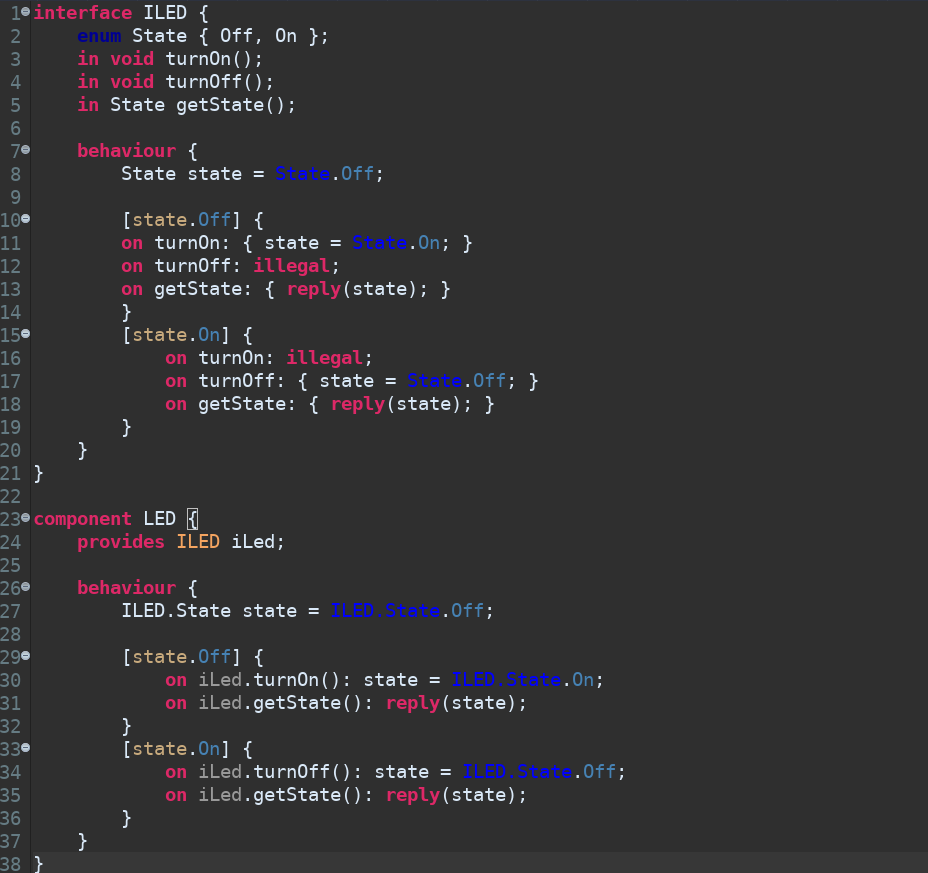
\includegraphics[width=\textwidth]{Figures/theoretical_background/enhanced_diagram.png}
    \caption{Dezyne model that turns a LED on and off}
    \label{fig:theoretical_background_dezyne_model}
\end{figure}

% TODO: Note no naming convention
First of all, notice the notions of an \textit{interface} and a \textit{component} from lines 1 to 21 and 23 to 38 respectively. Dezyne breaks logical control problems into components and interfaces. An interface defines the following: how a component interacts, the events that can be communicated and the interaction protocol (\cite{dzndoc}). In other words, it defines the behavior of a component, the events that it can execute and in what states it can execute those events. On line 2 we can see an enum declarion. This enum defines the states the system can be in. Below that, on lines 3 to 5 we see the event declarations of the system. Events are implemented as function calls in code (\cite{dzngloss}), as we will see in Section \ref{Generating code from a verified Dezyne model}. From line 7 to 20 we see the \textit{behaviour} block of the interface. Here we define in what states certain events are allowed, or what events should bring the system into a certain state. In this example we have chosen to declare behavior state-first, meaning we specify the state of the system first and then we specify which actions can occur in that state, but the language allows to declare behavior event-first as well, in which where we would specify the event first and then specify the states.
% Continue with turnOn turnOff getState, illegal, then component
On line 8 we declare that the system starts off in the \texttt{State.Off} state. Then on line 10 to line 14, we specify that when the system is in the \texttt{State.Off} state, we allow the \texttt{turnOn} and \texttt{getState} events to fire, but the \texttt{turnOff} is \texttt{illegal}, which as the keyword suggests makes the event illegal to fire. This makes sense, as when we are already in the \texttt{State.Off} state we cannot turn the system off. The \texttt{turnOn} event sets the state to \texttt{State.On}, and the \texttt{getState} event, using the \texttt{reply} keyword, return the current state of the system when the event fires. on lines 15 to 19 we specify what should happen when the system is in the \texttt{State.On} state. When the system is in the \texttt{State.On} state, the \texttt{turnOn} state firing should be illegal, as we cannot turn the system on when it is already on. The \texttt{turnOff} state turns off the system by setting the state to \texttt{State.Off}, and the \texttt{getState} event returns the current state of the event, just like when the system is in the \texttt{State.Off} state.
\\\\
We will now look at the component declared on lines 23 to 38. A component is a unit of definition and instantiation (\cite{dzngloss}). A component defines zero or more \textit{ports}, where a port is a named instance of an interface (\cite{dzngloss}). \texttt{provides} is the keyword used to define a port. In our example the defined port is \texttt{iLed}, an instance of the interface \texttt{ILED}. The idea of the behavior of a component is that it conforms to the behavior of its specification, or interface. We therefore make it start in the same state as the interface does on line 27. On line 29 to line 36 we specify the behavior of the component. Notice how, in this example, the behavior is the same, except that the events that are illegal are not specified. These need not be specified because the component infers what is illegal behavior from its provided interface. This is because verification of a component always goes through its interface, as we will see in Section \ref{Verifying a Dezyne model}. In this example the component's behavior block is almost exactly the same as the interface's behavior block. This is because the example is simple, more complex models will show more differences between the behavior blocks of the component of the interface. Nontheless, the behavior of the component should always conform to the behavior of the interface.
\\\\
Figure \ref{fig:led_example_graph} shows the state chart of our example LED model.

\begin{figure}[H]
    \centering
    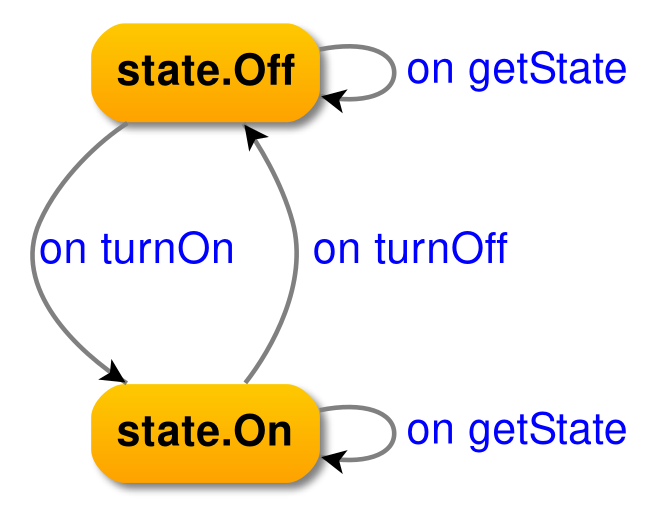
\includegraphics[width=0.5\textwidth]{Figures/theoretical_background/led_example_graph.png}
    \caption{State chart for the LED model}
    \label{fig:led_example_graph}
\end{figure}

In Figure \ref{fig:led_example_graph} we can see the \texttt{State.Off} and \texttt{State.On} states and  the \texttt{turnOn} \texttt{turnOff} and \texttt{getState} events we declared in code of the model in Figure \ref{fig:theoretical_background_dezyne_model}.

\subsection{Verifying a Dezyne model}
\label{Verifying a Dezyne model}
We will now look at the verification features of the Dezyne toolset. We will look at these features in context of the model in Figure \ref{fig:theoretical_background_dezyne_model}. Let us first verify the interface. When we verify the interface as it is given in Figure \ref{fig:theoretical_background_dezyne_model}, we get the message back that there are no verification errors in the interface. But things are not always so straightforward. Suppose that we forget to specify the \texttt{getState} event on line 13. If we then verify the model we will get the error message shown in Figure \ref{fig:not_specifying_all_events_error}.

\begin{figure}[H]
    \centering
    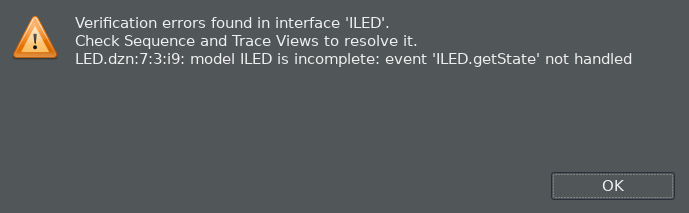
\includegraphics[width=0.7\textwidth]{Figures/theoretical_background/verification_of_interface_error.png}
    \caption{Interface verification error: Not specifying all events}
    \label{fig:not_specifying_all_events_error}
\end{figure}

The reason we get this verification error is that a well defined interface should specify the behavior of any of its declared interface, and that behavior should be specified for every state of the system. When we do not declare the \texttt{getState} event on line 13, we have not specified what behavior should take place if the \texttt{getState} event fires while the system is in the \texttt{State.Off} state.
\\\\
Let us return to the correct code as given in Figure \ref{fig:theoretical_background_dezyne_model} and let us now verify the component. The code of the component as it has been given in Figure \ref{fig:theoretical_background_dezyne_model} shows no first verification errors. In case a component gets through verification without errors we see a table like the one shown in Figure \ref{fig:Table showing no verifcation errors in the LED component}.

\begin{figure}
    \centering
    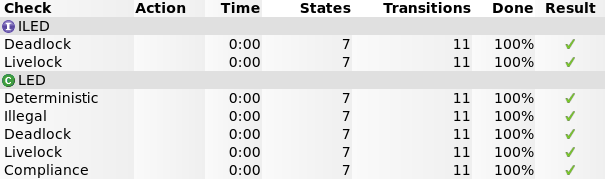
\includegraphics[width=0.8\textwidth]{Figures/theoretical_background/led_verification.png}
    \caption{Table showing no verification errors in the LED component}
    \label{fig:Table showing no verifcation errors in the LED component}
\end{figure}

In Section \ref{The Dezyne toolset and the Dezyne modelling language} we noted how verification of a component is always in context of its interface. We can see this fact in Figure \ref{fig:Table showing no verifcation errors in the LED component}, as interface \texttt{ILED} is first checked for deadlocks and livelocks before we check the \texttt{LED} component. The \texttt{ILED} interface shows no errors so the verifier goes on to the LED component. We can see that the component is checked for determinism, illegal statements, deadlocks, livelocks and compliance. Determinism in computer science refers to deterministic behavior of an algorithm. A deterministic algorithm is expected to produce the same output no matter what its input is (\cite{determinism}). The illegal statements refer to whether the component tries to execute an event that is deemed illegal by its provided interface. The definitions of deadlock and livelocks we have given in Section \ref{Terms and defintions}. Compliance refers to whether the component conforms to the behavior as specified in the interface.
\par
Let us now look at an instance of verification of a component where we get errors in the verification. Suppose we add the line: '\mintinline{c}{on iLed.turnOff(): state = ILED.State.Off;}' above line 30 in the code of Figure \ref{fig:theoretical_background_dezyne_model} to try and turn the LED off while it is in the off state. Since the interface the component provides does not specify that the \texttt{iLed.turnOff()} event can fire in the \texttt{State.Off} state, we get an error showing that the \texttt{iLed.turnOff()} event is not allowed by port iLed, as shown in Figure \ref{Component verification error: Not confirming to the interface}. Additionally, Dezyne shows a sequence diagram of a trace that leads to the error, as shown in Figure \ref{Sequence diagram showing that the component does not conform to the interface}. In this case, the trace is very short as the first event that executes, namely \texttt{turnOff}, is the cause of the problem.

\begin{figure}[H]
    \centering
    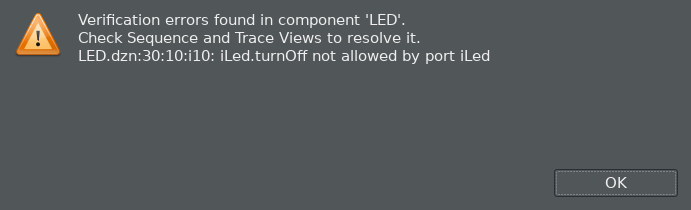
\includegraphics[width=0.7\textwidth]{Figures/theoretical_background/led_verification_error.png}
    \caption{Component verification error: Not confirming to the interface}
    \label{Component verification error: Not confirming to the interface}
\end{figure}

% TODO: Move this figure to the left
\begin{figure}[H]
    \centering
    
\includegraphics[width=\textwidth]{Figures/theoretical_background/verification_error_in_sequence_diagram.png}
    \caption{Sequence diagram showing that the component does not conform to the interface}
    \label{Sequence diagram showing that the component does not conform to the interface}
\end{figure}

From this we can see that the interface prevents us from executing actions (events) that are not allowed by it. Let us remove the \texttt{turnOff} action, so that we end up with the code in from Figure \ref{fig:theoretical_background_dezyne_model} again. Suppose we removed line 35: \texttt{on iLed.getState(): reply(state)}, because we do now want to be able to get the state when the LED is in the \texttt{State.On} state anymore. If we then verify the model, we get an error saying that getState is an implicitly illegal action, as we can see in Figure \ref{Component verification error: getState implicitly illegal}. The accompanying sequence diagram is shown in Figure \ref{Sequence diagram showing that the component does not conform to the interface}.

\begin{figure}[H]
    \centering
    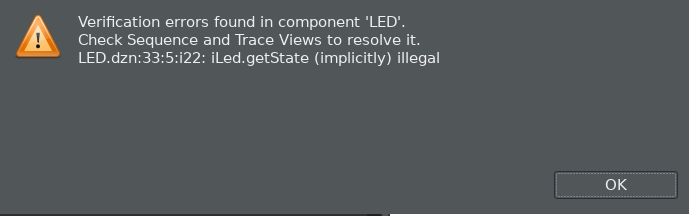
\includegraphics[width=0.7\textwidth]{Figures/theoretical_background/led_verfication_error_getState.png}
    \caption{Component verification error: getState implicitly illegal}
    \label{Component verification error: getState implicitly illegal}
\end{figure}

\begin{figure}[H]
    \centering
    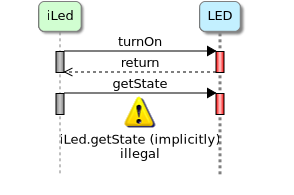
\includegraphics[width=0.5\textwidth]{Figures/theoretical_background/getState_implicitly_illegal.png}
    \caption{Sequence diagram showing that getState is an illegal action in the component}
    \label{Sequence diagram showing that the component does not conform to the interface}
\end{figure}

The reason we get the error shown in Figure \ref{Component verification error: getState implicitly illegal} and Figure \ref{Sequence diagram showing that the component does not conform to the interface} after removing line 35 is because not specifying an event means that the event is illegal in Dezyne. But this is in contrast to what we specified in the \texttt{ILED} interface. We did not specify that \texttt{getState} is illegal in the interface, therefore the error says that \texttt{getState} is \textit{implicitly} illegal.
\par
The takeaway from this example is that a component must always conform to what is specified in its provided interface.
\\\\
% TODO: Add ref
Lastly, let us look at a sequence diagram for the correctly verified model of Figure \ref{fig:theoretical_background_dezyne_model}. The sequence diagram is shown in Figure \ref{Sequence diagram of the LED component}. This is also called a simulation in Dezyne, because we simulate the system's control logic, taking a particular walk through the available actions. At the bottom of the figure we can see the particular actions we can execute, that is, events that can fire in this system's state, and on the right we see a watch window that shows values of the variables of the interface and the component. Since this example consists of just a \texttt{LED} component and its interface, the sequence diagram does not give us much information that we could not already deduce from the state diagram in Figure \ref{fig:led_example_graph}. However, for more complex systems like our safety module given in \ref{}, the sequence diagrams will prove to be a very useful visualisation of the system.
\\\\
In the next section we will look at the C++ code we can generate from our LED example model.

\begin{figure}[H]
    \centering
    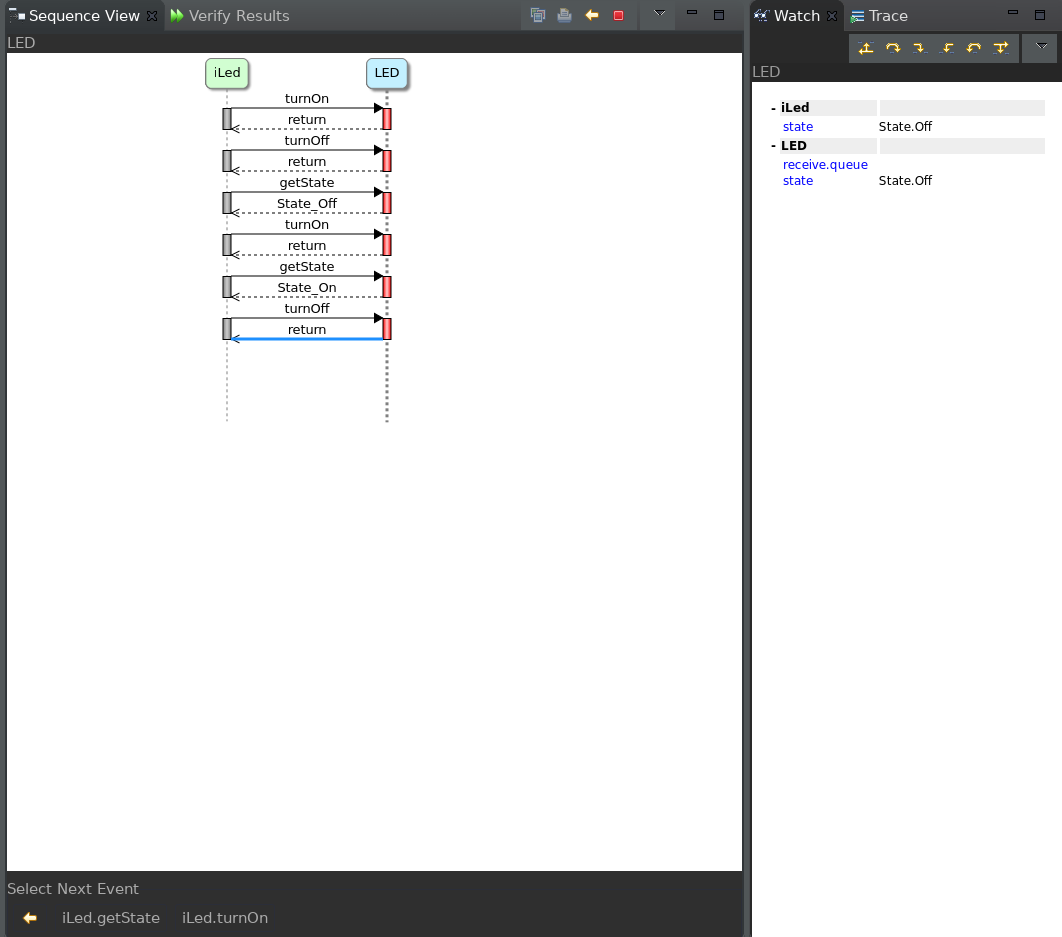
\includegraphics[width=\textwidth]{Figures/theoretical_background/simulation_of_led.png}
    \caption{Sequence diagram of the LED component}
    \label{Sequence diagram of the LED component}
\end{figure}


\subsection{Generating code from a verified Dezyne model}
\label{Generating code from a verified Dezyne model}
    In this section we will look at the code generation feature of Dezyne. We will make use of the model from Figure \ref{fig:theoretical_background_dezyne_model} for the generation of the code. To make the demonstration simpler, instead of letting the \texttt{turnOff} and \texttt{turnOn} events be illegal on lines 12 and 16, we simply switch the state to \texttt{State.Off} and \texttt{State.On} respectively. we also added those actions to the component. Furthermore, to demonstrate the system component, which will be useful in code generation, we added a \texttt{IController} interface, a \texttt{Controller} component and a system component above the \texttt{ILED} interface. These additions are shown in Figure \ref{Addition of interface IController, component Controller and system component}. The system component generates a System view which is shown in Figure \ref{System view of the controller and led system}.
    
\begin{figure}[H]
    \centering
    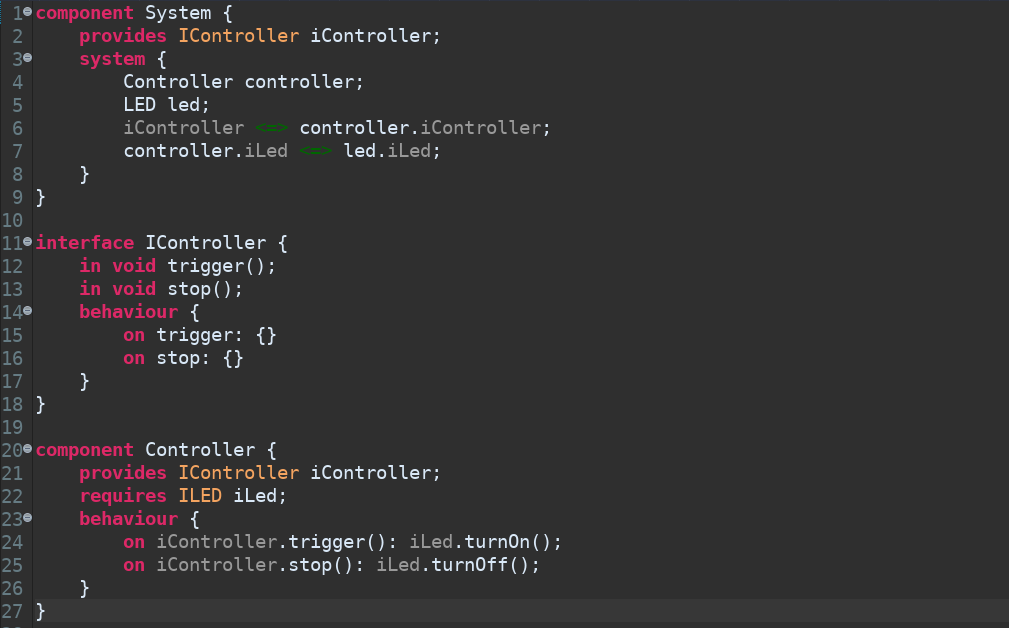
\includegraphics[width=\textwidth]{Figures/theoretical_background/system_component.png}
    \caption{Addition of interface IController, component Controller and system component}
    \label{Addition of interface IController, component Controller and system component}
\end{figure}

\begin{figure}[H]
    \centering
    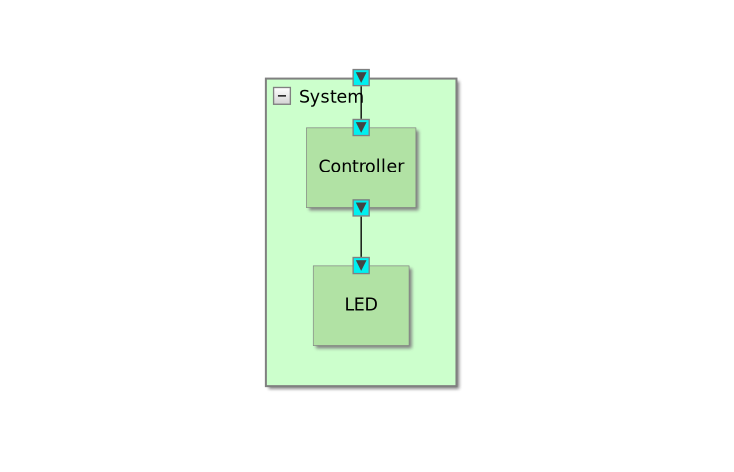
\includegraphics[width=0.9\textwidth]{Figures/theoretical_background/sys_view.png}
    \caption{System view of the controller and LED system}
    \label{System view of the controller and led system}
\end{figure}

The Controller's job is to simply turn the led on and off with its \texttt{trigger} and \texttt{stop} functions. We can see that it does that by calling the \texttt{iLed.turnOn} and \texttt{iLed.turnOff} events. In line 22 of Figure \ref{Addition of interface IController, component Controller and system component} we specified that the controller component will call events from \texttt{ILED} with the \texttt{requires} keyword. In the component called \texttt{System} we see some more new syntax.  The system section, as indicated by the keyword \texttt{system}, consists of two parts: instantiations of subcomponents, followed by all the bindings among the sub-components and ports of the component. This results in the system view shown in  Figure \ref{System view of the controller and led system}. This system view shows all the components of the system. We will see how the system view is useful to us in the generated code shortly.
\\\\
% TODO: Add appendix
We will now generate source code from the model. Dezyne provides the option to generate code in a variety of languages. For this example we choose to generate C++ code, as C++ is the language used for the safety module as well. In Listing \ref{lst:led_example code} we show a very minimal main function to use the generated code and Figure \ref{Execution of minimal led example code} shows the execution of the compilation of this code. The generated code itself can be found in Appendix \ref{}.

\begin{listing}[ht]
\begin{minted}[mathescape,
               numbersep=5pt,
               frame=lines,
               framesep=5mm,
               linenos]{c}
               
#include <iostream>
#include <dzn/runtime.hh>
#include <dzn/locator.hh>
#include "LED_example.hh"

int main() {
    dzn::locator loc;
    dzn::runtime rt;
    loc.set(rt);
    System s(loc);
    s.dzn_meta.name = "LedExampleSystem";
    s.check_bindings();

    std::string input;
    while(1) {
        std::cin >> input;
        if (input == "On")
            s.iController.in.trigger();
        else if (input == "Off")
            s.iController.in.stop();
    }
    return 0;
}

\end{minted}
\caption{Example source code}
\label{lst:led_example code}
\end{listing}

\begin{figure}[H]
    \centering
    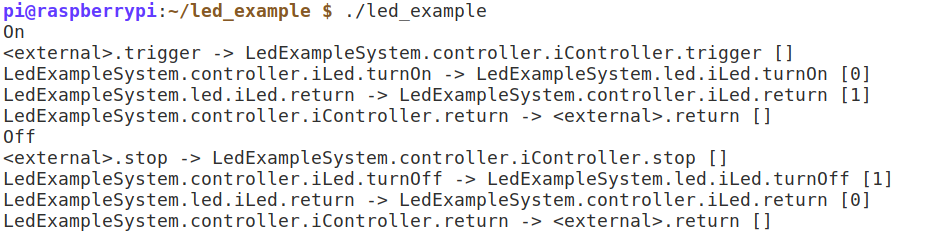
\includegraphics[width=\textwidth]{Figures/theoretical_background/executed.png}
    \caption{Execution of minimal led example code}
    \label{Execution of minimal led example code}
\end{figure}

%TODO: Add ref
Lines 7 to 11 concern the allocation and use of the Dezyne runtime. Usage of the Dezyne runtime is elaborated extensively in the documentation of the toolset (\cite{dzndoc}). On line 10 we declare a system object. The system object is useful because we can use it to check whether every function from dezyne is bound to a function in our C++ code and we can access our dezyne functions, \texttt{trigger} and \texttt{stop} through it, as is done on line 18 and line 20 respectively. In our simple example we have not bound any Dezyne functions to C++ code. In a real system we would bind the LED's \texttt{turnOn} and \texttt{turnOff} events to C++ functions that are able to turn a real LED on and off. Examples of the binding of Dezyne events to functions can be found in the documentation or in our Results on the modelling of the safety module in Section \ref{}. 
\par
The executed code in Figure \ref{Execution of minimal led example code} shows how we simulate turning on and off a LED by giving the program the input \texttt{On} and \texttt{Off}. We can see that the controller calls \texttt{iLed.turnOn} and \texttt{iLed.turnOff} internally as we call \texttt{iController.trigger} and \texttt{iController.stop}.
\\\\
There are many useful features of Dezyne we have not discussed. For example, the Dezyne runtime actually prevents you from calling events declared illegal. Moreover, components implemented in source code can inherit skeleton classes to make sure every function that needs an implementation is actually implemented. Many examples are given in (\cite{dzntut}) and many of the features we use in our model of the safety module. The strength of the toolset really comes from the ability to carry over the verification of the model to the implementation code, making sure that what we verified stays correct in the implementation.


\chapter{Results}
TODO\\
O\\
D\\
O\\
In this chapter we present the results of our research. First we will present our choice of hardware and choice of operating system.
\par
All code and documentation can be found in \href{https://github.com/Yousousen/safety-module-for-care-robot-rose.git}{our github repository}.
%    • weergave van de resultaten
%    • beschrijving toe te passen theorie (let op: dit betekent dat er een deelvraag is die over de theorie gaat)
%    • bespreek de resultaten in een logische volgorde (per deelvraag)
%    • alleen relevante tabellen en overzichten (minder relevante tabellen en overzichten neem je op in de bijlagen)
%    • de resultaten nog niet interpreteren, dat komt in het hoofdstuk Conclusie 

\section{Choice of hardware and operating system}
\label{Choice of hardware and software}
%This section describes the choices made for the hardware of the safety module. First the main requirements of the hardware are listed. Then a comparison is made between available hardware solutions which can be used to implement the safety module. \\
In this section we elaborate on the hardware and software choices that were made for the assignment.

\subsection{Main component}
\label{Main component}
% TODO: ref to specification of Rose
We will now look at the choices made for the hardware of the safety module. We will first look at the main component. The main component of the safety module specifies the heart of the system; the CPU, RAM, and related peripherals. In Chapter \ref{Theoretical Background} we explored previous research to see what others have used as their main component. In Section \ref{tHardware} we saw that \citeauthor{delgado} used a Raspberry Pi 3 in their control architecture on their mobile service robot. In Section  \ref{tHardware} we also noted that previous research describes the main component of the robot itself, while in our research the main component of the robot already exists; namely the robot, Rose, has two Ubuntu systems, \texttt{rosepc1} and \texttt{rosepc2} which together form the main component of the system, consisting of the CPU, RAM and related peripherals. \texttt{rosepc1} and \texttt{rosepc2} are connected to the grip arm Rose uses to grab items with, the kinect camera Rose uses to see her environment with and the WiFi router which connects Rose to her operator. \texttt{rosepc1} and \texttt{rosepc2} correspond with what \citeauthor{bouchier} described as the first architecture in \ref{tHardware}, a complete Linux distribution, but without real-time patches or a real-time framework. The safety module we implement in this research is an addition to the already existing system of Rose.\\

We will now look at available hardware solutions to determine what is the best choice for the main component of the hardware based on the requirements listed in Section \ref{Assignment specification}.
\\
The \gls{pi} is a small computer with various software solutions for real-time computing. Raspbian, the default operating system of the \gls{pi}, is an operating system based on Debian, a Linux based operating system. The Linux kernel can be configured for real-time computing through the \mintinline{c}{CONFIG_PREEMPT_RT} parameter (\cite{rtwiki}) and by use of a scheduler with priority queues (\cite{linux_scheduling}). Another option is to configure the Linux kernel for real-time computing is to use the Xenomai project framework, which is an open source software project aiming to build a real-time framework for Linux (\cite{xenomai}). 
\par
The \gls{pi} offers support for the addition of peripherals through its 40 pins GPIO header. It has a build in WiFi module and Ethernet interface. Various resources on the internet provide guides for embedding a \gls{pi} in a project, and the \gls{pi} Foundation (\cite{foundation}) offers clear documentation on the available features of the \gls{pi}. The Linux kernel and the Xenomai project offer thorough documentation as well. Our literature study in Section \ref{tHardware} showed that multiple studies used a \gls{pi} in their mobile robotic applications. These options will be compared in Section \ref{Operating System}.
\\\\
The Arduino Uno is a \gls{mcuu} board based on the Atmel 8-bit ATmega328P \gls{mcuu} (\cite{arduinouno}). The board provides an usb interface to program the \gls{mcuu} without the need of a \gls{mcuu} programmer and contains various other utilities to ease interaction with the \gls{mcuu} on the board. Through the use of ARTe (Arduino Real-time extension) the Arduino Uno can be extended to support multitasking and real-time preemptive scheduling (\cite{ARTe}). At the time of writing,  the real-time extension for the Arduino framework lacked up-to-date and clear documentation however. Just like the \gls{pi}, the newest version of the Arduino Uno has build in \gls{wifi} module. In Section \ref{tHardware} we saw that \cite{arduino} used an Arduino in their robotic control system.
\\\\
In Section \ref{tHardware} we also found that \gls{mcuu} are used in robotic applications. Microcontrollers like the Microchip PIC series can be used for real-time systems as they are highly configurable which  allows them to fit well to the needs of a project. (\cite{micro}) The programmer can program the task scheduler of the \gls{mcuu} himself to fit the needs of the system. Microchip offers an extensive feature lists in their datasheets of the various \gls{mcuu}s they offer. A disadvantage for usage of a \gls{mcuu} in this project is that a \gls{mcuu} has no build in \gls{wifi}, \gls{4g}, and ethernet module which means these need to be added in addition to the measuring devices required for the project. Furthermore, because \gls{mcuu}s generally do not run an operating system, considerable time has to be put into developing a scheduler for the \gls{mcuu}.
\\\\
To make a decision for the main component of the hardware we set up a table to compare the components and see how well they fit in fulfilling the requirements listed \ref{Hardware setup}. As a first selection we chose the \gls{pi} 3B+, the Arduino Uno SMD R3 and the PIC16F15386 \gls{mcuu}. Earlier this section we described why the \gls{pi} and Arduino Uno are good choices. The PIC16F15386 we selected because Microchip recommends it for real-time applications (\cite{micro}).  In Table \ref{hardware_table}, all three components have been given points based on how well they fit the requirements and their advantages and disadvantages. They get a score of 1 if they fit the requirement not very well, 2 if they fit well enough, and 3 if they fit the requirement very well. The component with the largest total points will be chosen as the main component for the hardware. We left out Requirement \ref{hsTwo}, the requirement that the hardware should be able to communicate with \acrshort{ros}, as all components support this. We also left out Requirement \ref{hsFive}, for all components are lightweight and small. Lastly we estimated the total cost after addition of peripherals and scored gave a score for their price. Table \ref{hardware_table} shows the results.

\begin{table}[H]
    { \rowcolors{3}{magicmint}{paleblue}
    \begin{tabularx}{\textwidth} { 
      | >{\raggedright\arraybackslash}X 
      | >{\raggedleft\arraybackslash}X 
      | >{\raggedleft\arraybackslash}X 
      | >{\raggedleft\arraybackslash}X | }
      \hline
      \rowcolor{mediumturquoise}
     \multicolumn{4}{|c|}{\large Main component comparison} \\ \hline
     & \gls{pi} 3B+ & Arduino Uno SMD R3 & PIC16F15386 \acrshort{mcu} \\ \hline
     Real-time support & 3 & 1 & 3 \\ \hline
     Ethernet support & 3 & 3 & 1 \\ \hline
     \gls{wifi} and \gls{4g} support & 3 & 2 & 1 \\ \hline
     Peripheral support & 3 & 3 & 3 \\ \hline
     Estimated total costs & 2 & 2 & 3 \\ \hline
     Total score & 14 & 11 & 11 \\ \hline  
     %\label{hardware_table}
    \end{tabularx}
    }
    \caption{Table to compare potential hardware choices}
    
    \label{hardware_table}
\end{table}

% TODO: Euro sign here
We gave the Arduino Uno SMD R3 only one point for \textit{real-time support} because at the time of writing we found the documentation for the real-time framework to be unclear and outdated. We gave the PIC16F15386 \gls{mcuu} 1 point for \textit{\gls{wifi} and \gls{4g} support} because it requires a lot of development time relative to the Arduino Uno and \gls{pi}. The PIC16F15386 has three points for \textit{estimated total costs} because it is cheaper than the other two. None of the choices exceeded the maximum of €300,-, with all three choices averaging below €100,-.
\par
The last row shows the total score of each component. We can see that the score \gls{pi} 3B+ scored the highest, we therefore think the \gls{pi} 3B+ is the best choice for the main component of the safety module.

\subsection{Measuring devices}
Having chosen on the main component of the safety module system in Section \ref{Main component}, we looked into measuring devices for the \gls{pi} to fulfill Requirement \ref{hsFive} listed in Section \ref{Hardware setup}, namely the addition of an accelerometer for measuring acceleration and gyroscope for measuring angular velocity.
\par
There are various options to add additional measuring devices to the \gls{pi}. One option is to buy the devices separately. Another option is to buy an add-on board commonly called a \gls{pi} HATs with multiple sensors on it. We went for the second option, as it greatly decreases development time and is extensible for future releases of the safety module. We chose the \gls{pi} Sense HAT, as it was the most readily available \gls{pi} HAT that contained both an accelerometer and a gyroscope. In addition to this, the \gls{pi} Sense HAT has a number of advantages over using separate measuring devices:

% TODO: Add ref to library explanation
% TODO: Perhaps elaborate the LED matrix part.
% TODO: Perhaps remove the ref.
\begin{itemize}
    \item The Sense HAT has a magnetometer for measuring the magnetic field at a particular location
    \item The Sense HAT can fuse accelerometer, gyroscope and magnetometer data to reduce uncertainty in measurements.
    \item The Sense HAT comes with a library that can be used to receive data from the sensors on the Sense HAT. We will elaborate the usage of this library in Section \ref{}.
    \item The Sense HAT has a LED matrix which can be used to show the results of safety checks.
\end{itemize}

Furthermore, the Sense HAT has a humidity sensor, a  pressure sensor and an on board joystick. These are not needed for the prototype of the safety module, but could be useful for further releases of the safety module. For example, the joystick can be used for adding minimal control support for when the joystick of Rose her operator does not work. The humidity sensor and pressure sensor could be used to get more detailed information on the environment a care robot is located in.
\par
% TODO: ref to the chapter 2 section where that is described.
Figure \ref{sensehat} shows the sense HAT. The components of interest for us in this research are the the inertial measurement unit (IMU), labeled \texttt{ACCEL/GYRO/MAG}, which contain the accelerometer, the gyroscope and the magnetometer, and the LED matrix. The name of the IMU itself is \textit{LSM9DS1}. Figure \ref{} shows the orientation of the IMU. The orientation is such that if we lay down the \gls{pi} with Sense HAT attached in front of us, in such a way that the Ethernet port points towards us, then that is the direction labeled X. As we can see, the Z direction denotes the up -down direction, and the only other direction left is the Y direction. The fact that we live in a universe with three spatial dimensions complicates the way we want to measure acceleration a bit. The measuring of the quantities of acceleration and angular displacement will be elaborated in Section \ref{}.

\begin{figure}[H]
    \centering
    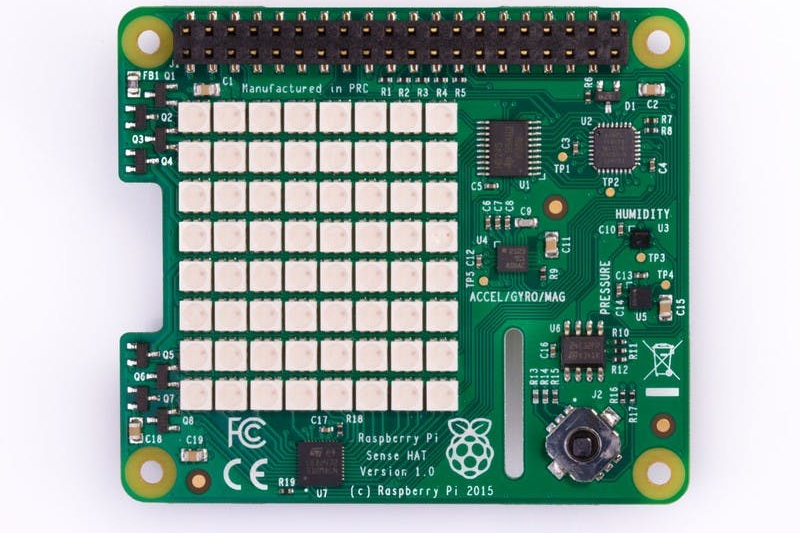
\includegraphics[width=0.5\textwidth]{Figures/results/sense_hat_correct.jpg}
    \caption{Raspberry pi sense hat, source: \cite{sensehat}}
    \label{fig:sensehat}
\end{figure}

\begin{figure}[H]
    \centering
    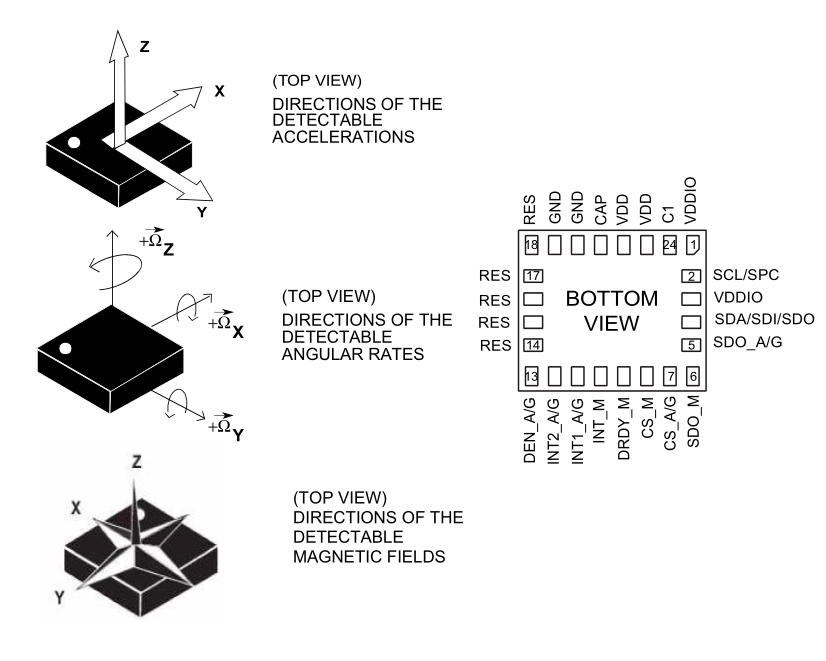
\includegraphics[width=0.5\textwidth]{Figures/results/imu_orientation.png}
    \caption{Axis of the IMU. source \cite{lsm9ds1}}
    \label{fig:imu_orientation}
\end{figure}

\subsection{Operating System}
\label{Operating System}
In our literature review in Section \ref{tOS} we saw that Linux distributions are often used in care robot systems, because ROS is a popular middleware and ROS runs best on Linux distributions. We choose to run a Linux distribution on the \gls{pi} of the safety module, because care robot Rose runs ROS as well, and the safety module needs to interact with care robot Rose. Specifically, we choose to run Raspbian, the Debian based Linux distribution for the \gls{pi}, as it is optimized for the \gls{pi}'s hardware (\cite{raspbian}).
\par
As was shortly mentioned in the description of the \gls{pi} in Section \ref{Main component} and as was elaborated in detail in the literature review of Section \ref{tOS}, the two prominent options for adding real-time support to Linux distributions are real-time Linux and the Xenomai framework. In Section \ref{tOS} we also saw a comparison between these two options, with as result that Xenomai performed better in terms of meeting hard real-time requirements. Now, for the prototype safety module that is developed in this research, we only aim for soft real-time performance. Still, further versions of the safety module will need to support hard-real-time performance, and we therefore choose to use the cokernel setup of the Xenomai framework over Real-time Linux as our operating system.
\par 
% TODO: Gloss system call
As was shortly mentioned in Section \ref{tOS}, Xenomai provides various skins. These skins are interfaces to the real-time functionality that the Xenomai framework provides. We choose to work with the POSIX skin. The POSIX skin provides the functionality of the Xenomai framework through the interface of a subset of POSIX system calls. The following services are provided (\cite{posix_xenomai}):

\begin{itemize}\label{posix_wrapped}
    \item Clocks and timers
    \item Condition variables
    \item Message queues
    \item Mutual exclusion 
    \item Process scheduling 
    \item Semaphores
    \item Thread management
    \item Scheduling management
\end{itemize}

These POSIX services are wrapped around with Xenomai versions of the calls. For example, if one calls the \mintinline{c}{pthread_create} function to create a new thread in the C or C++ programming language, what is actually called is a real-time implementation of the system call provided by the Xenomai framework.
\par
% TODO: Ref to results S4
The reason we choose to work with the POSIX skin as opposed to other skins is that the POSIX skin avoids the need to rewrite device drivers written for standard, non-Xenomai Linux, as such device drivers often use the POSIX services given in the previous. In our case this avoids the need to rewrite the driver for the Sense HAT. Likewise, \acrshort{ros} is targeted for standard Linux and not Xenomai, so using the POSIX skin also avoids having to rewrite \acrshort{ros} services. Section \ref{} shows how we implemented the safety module using the xenomai framework.
\\\\
We have built \acrshort{ros} for Raspbian and installed it on our system. For this research we will simulate interaction with care robot rose and ROS and will not use this installation, however. The reason we installed \acrshort{ros} is to show the feasibility of using the system of the \gls{pi}, raspbian with xenomai as a whole.
\par
% TODO: ref to dezyne chapter.
Figure \ref{} gives a high overview of this system as a whole, visualised as a stack. On the bottom we have the \gls{pi} with the Sense HAT, this denotes our hardware. On top of that we have got the Linux kernel and the Xenomai cokernel, which run besides each other. Then we have got Raspbian Buster, the operating system. On top we see RTIMULib, Dezyne and \acrshort{ros}. RTIMULib is the library used to communicate with the sense hat. Dezyne is the modelling language we use, which uses its own runtime library. The use of Dezyne is elaborated extensively in its own chapter, Chapter \ref{}. The reason RTIMULib and \acrshort{ros} are shown on top, despite the fact that both communicate with the hardware of the bottom layer, is because RTIMULib and \acrshort{ros} are both libraries called from user space. We can say that anytime we want to access a hardware device in our proram we traverse the stack from top to bottom.

\begin{figure}[H]
    \centering
    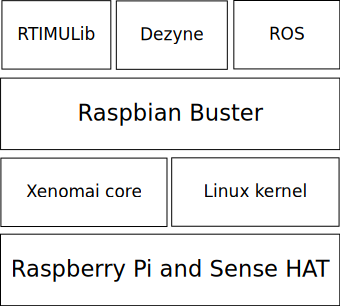
\includegraphics[width=0.5\textwidth]{Figures/results/os_environment_stack.png}
    \caption{Safety module system stack}
    \label{fig:my_label}
\end{figure}


% TODO: ref to section
%       fix list reference (actually ref to the list and not the section.
Let us look at a communication scheme of the system and how the Xenomai framework provides us with real-time operation of the safety module. In Figure \ref{fig:communication_scheme} an overview of the communication scheme of the system is given. On the left side we can see our program and the Xenomai core. These are are in \textit{primary mode}, primary mode is the real-time domain; the part of the system that operates real-time, because it is governed by the Xenomai cokernel. This is due to that all scheduling of tasks in primary mode is handled by the Xenomai core. The Xenomai framework provides us with the ability to make a subset of system calls, the ones from the items listed in List \ref{posix_wrapped} without leaving primary mode. We depicted Dezyne to be inside our program, in primary mode. The code that Dezyne generates from the model is essentially the control loop of the safety module system. This control loops executes five checks, this is why there are five lines of communication going through the entire system in the overview of Figure \ref{fig:communication_scheme}. These checks are checks on five aspects of the robot: the kinetic energy, the rotational energy , the grip arm strength, both force and torque, and grip arm position. These checks are elaborated extensively in the subsequent Results sections. RTIMULib and ROS communicate with device drivers written for the standard Linux kernel, meaning they do not run in primary mode, but \textit{secondary mode}. Secondary mode is the non-real-time domain; the part of the system that does not operate in real-time and is governed by the standard Linux kernel. This brings us to a problem. Our program needs to communicate with these libraries, and therefore with these device drivers, but if it does so it would make a mode switch by moving from primary mode to secondary mode. One solution would be to reimplement all used device drivers to work with the xenomai framework, so that they can run in primary mode. This solution, however, takes a lot of development time and research into how to convert standard linux drivers to real-time drivers. Luckily, Xenomai provides us with another solution: the use of XDDP sockets. XDDP sockets allow the part of the system running in primary mode to communicate data with the part of the system running in secondary mode, without the former leaving primary mode. This is good because now we can set up the system as follows. In primary mode the control loop runs in real-time governed by the Xenomai cokernel. In secondary mode, threads retrieving data from the sensors are running and provide their data on the XDDP socket, which can then be read by the threads of the program running in primary mode. This set up gets rid of the problem of our control loop needing to leave primary mode to access sensor data. However, now, there is another problem luring in the background. What should we do when the sensor data is not provided by the non-real-time thread when a real-time thread requires it? We go into more detail on this problem in Section \ref{}, but essentially the real-time checks just keep going regardless of whether there is data provided by the non-real-threads. That is to say, the checks do not block if there is no data available.

\begin{figure}[H]
    \centering
    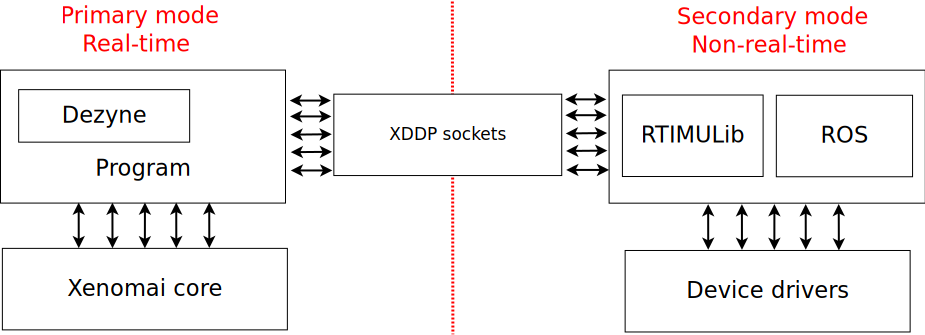
\includegraphics[width=\textwidth]{Figures/results/communication_scheme.png}
    \caption{Distinction between primary mode and secondary mode}
    \label{fig:communication_scheme}
\end{figure}

\section{Retrieving and Using Sensor Data}
In this section we elaborate our results on how to retrieve sensor data and use this data to check whether the safety module has performs unsafe actions.
\par
In Section \ref{Assignment specification} we defined unsafe behaviour as behavior that could result in injury to humans or damage to the environment by collision, clamping or pinching of the care robot with an object or human. The goal of the safety module is to provide a second layer of safety checks upon the already existing safety checks by the care robot itself. In Section \ref{Safety in care robots} we explored the how existing research measures safety in robots. We implement a rudimentary form of some of these safety checks by looking at four aspects of the care robot. These are: its kinetic energy, its rotational energy, its grip arm strength and the position of the grip arm. These aspects were given on the Risk Analysis for additional safety measures of robot Rose (\cite{risk_analysis_additional}).

\subsection{Sensors on the safety module}
The sensors of the Sense HAT of the safety module are used to check the kinetic energy and rotational energy of the robot. The safety module is attached to the care robot, and should be attached in a way such that the x-axis (see Figure \ref{fig:imu_orientation}) points forward.
\par
We make use of the RTIMULib library, an open-source library that provides us an application programming interface (API) to interact with the accelerometer, gyroscope and magnetometer of the LSM91DS1, the inertial measurement unit of the Sense HAT \cite{rtimulib}. With the use of a Kalman-filter the library provides fused data of the accelerometer, gyroscope and magnetometer. Kalman-filtering is a technique to provide an accurate measure of, in our case, the angular orientation of the safety module.

\subsubsection{Kinetic energy}
\label{Kinetic energy}
First we will look at the aspect of kinetic energy. In classical mechanics, kinetic energy is defined as follows:

\begin{equation} \label{eq:ke}
    E_k = \frac{1}{2}mv^2
\end{equation}

where $m$ is the mass and $v$ the velocity of the object undergoing linear translation. Robot Rose's mass is $95kg$ (\cite{rose_specification}), the \gls{pi}'s mass is $45g$ (\cite{raspberry_pi_weight}) and the Sense HAT's mass is $20g$ (own measurement). That gives us $m = m_{tot} = 95.65kg$. Velocity we do not measure directly, instead we measure the acceleration using the accelerometer on the Sense HAT. To obtain velocity $\vec{v}$ from acceleration $\vec{a}$, we numerically integrate $\vec{a}$ using the following equation:

\begin{equation} \label{eq:trapezoidal_rule}
    \vec{v} = \int_{t_0}^t \vec{a}\ dt \approx \sum_{t=1}^{N} \frac{\vec{a}(t-1) + \vec{a}(t)}{2}\Delta t
\end{equation}

where $N$ is the number of samples, and $\Delta t$ is a small change in time. Equation \ref{eq:trapezoidal_rule} is called the \textit{Trapezoidal rule}. For larger $N$ and smaller $\Delta t$ the approximation becomes more accurate. We have determined an appropriate value for $N$ and $\Delta t$ such that the time taken to sample the acceleration is proportional to the recommended poll interval of the IMU as given by RTIMULib.
\par
Various sources report the occurrence of drift error due to sensor noise by using integration to obtain velocity from acceleration (\cite{chrobotics}) (\cite{googletechtalks}) (\cite{Woodman07anintroduction_oliver}). For the double integration that is done to obtain position the error is even worse. However, we can still use this method of determining velocity for our purposes, for the obtained velocity is accurate enough to determine kinetic energy and we discard the value of velocity after determining the kinetic energy gained from it. Every time we calculate the kinetic energy, we do so by obtaining the kinetic energy that is gained from the change in acceleration, that is to say, our error does not get increasingly worse, because we only measure changes in acceleration and do not take into account the velocity the robot may already have.
\par
A subtle, but important point that follows from this, is that we do not actually measure the kinetic energy of the robot, but the change in kinetic energy. Furthermore, with discarding the previous value of velocity we mean we set the initial velocity to be zero every time we want to calculate the kinetic energy. So the following equation holds:
\\\\
% TODO: ref recommendations

\begin{equation} \label{eq:change_ke}
    \Delta E_k = \frac{1}{2}m(\Delta v)^2 \implies \Delta E_k = \frac{1}{2}mv^2,\quad if\ \vec{v_i} = 0
\end{equation}

where $\Delta v$ is the change in velocity and $\vec{v_i}$ is the initial velocity.
\par
% TODO: tHardware ref correct here?
Excessive change in kinetic energy will cause the robot to collide with a human or object, which we defined as a form of unsafe behavior. To avoid this, the obtained change in kinetic energy is compared to the maximum allowed change in kinetic energy. For our purposes, this maximum allowed change in kinetic energy is the same for every situation. The maximum allowed change in kinetic energy is given as input to the safety module either in a file or as command line argument. The value is not determined by us, but by the company or organisation who employs the safety module, who has tested and determined an appropriate value for this variable. We have chosen a value that most clearly demonstrates the use of the check on kinetic energy.

\subsubsection{Rotational energy}
\label{Rotational energy}
The rotational energy is determined similarly to the kinetic energy, but using angular variables instead, and we calculate the actual rotational energy, not the change in rotational energy. The rotational energy is calculated using the following equation:

\begin{equation}
    %\Delta E_{rot} = \frac{1}{2}I(\Delta\omega)^2 \implies \Delta E_{rot} = \frac{1}{2}I\omega^2,\quad if\ \vec{\omega_i} = 0
    E_{rot} = \frac{1}{2}I\omega^2
\end{equation}

where $I$ is the moment of inertia and $\omega$ is the angular velocity. For $I$ we approximate the robot as if it were a solid cylindrical object. $I$ can then be calculated as follows:

\begin{equation}
    I = \frac{1}{2}mR^2
\end{equation}

where $m$ is the mass of the robot and $R$ the radius of the robot. $R$ we approximate to be 1 meter, taking the scenario into account where Rose fully stretches her arm.
\par
The fused accelerometer, gyroscope and magnetometer data gives us an accurate measure of the angular displacement $\vec{\theta}$ of the safety module. With $\vec{\theta}$ we can calculate the angular velocity $\vec{\omega}$ using numerical differentiation as follows:

\begin{equation}
    \vec{\omega} = \frac{d\vec{\theta}}{dt} \approx \frac{\Delta\vec{\theta}}{\Delta t} = \frac{\vec{\theta}(t + \Delta t ) - \vec{\theta}(t)}{\Delta t}
\end{equation}

Here $\Delta t$ is a small change in time, which is, just like the $\Delta t$ used in the determinatino of the velocity in Section \ref{Kinetic energy}, proportional to the poll rate of the IMU.
\par
Excessive rotational energy will cause the linear momentum of the robot to be too great when it rotates, which results can result in damage to the environment or injury to humans. Therefore, just like with kinetic energy the rotational energy is compared to a maximum allowed value.

\subsection{Sensors on robot Rose}
Ultimately, Rose's arm sensors will be used to retrieve the strength and position of the arm. These values are received from \acrshort{ros}. ROS provides a publisher-subscriber type of pattern in which a subscriber can listen on a \textit{topic} on which the publisher publishes data. In our case the subscriber would be the safety module and the publisher would be Rose. Topics in ROS are just a collection of messages concerning a particular subject, where a message is the means of communication of data in \acrshort{ros} (\cite{agitr}).
\par
Currently we use generated values from within the safety module itself and do not communicate with robot Rose through \acrshort{ros}. We have still installed ROS on the safety module to show the feasiblity of the system as a whole. Documentation on the installation of ROS on the safety module can be found on \href{https://github.com/Yousousen/safety-module-for-care-robot-rose.git}{our github repository}.
\subsubsection{Force and torque}
Strength can be expressed in two different kind of forces. One is the force of the arm against an object, the other is a rotational force, commonly called \textit{torque}, that is used to grab an object. We need not calculate the force and torque like we did with kinetic energy and rotation energy, because ultimately care robot Rose provides these values through \acrshort{ros}.
\par
Excessive force can cause the arm to clamp with an object, and excessive torque can cause the arm to pinch an object. Both are cases we want to avoid. We, therefore, just like with kinetic energy and rotational energy, set a maximum allowed value for the force and torque, which should not be exceeded.

\subsubsection{Position}
The last check on unsafe behavior concerns the arm position of the robot. When the robot is moving, the arm should be in a folded position. This means it is not stretched, and in a position that it can do the least amount of harm. This value, too, is ultimately provided by Rose through \acrshort{ros}, and need not be calculated by the safety module.

\subsection{When the result of a check gives unsafe behavior}
% TODO: ref to modelling section.
What should we do when a check is executed and the maximum allowed value for the kinetic energy, rotational energy, force, torque is exceeded, or when the arm is not folded when the robot is moving? 
These are the situations we call unsafe behavior. In such a case, the LED matrix receives a signal to turn red. On default, the LED matrix is low. When a check is executed and the result of the check is that there is no unsafe behavior, the LED matrix receives a signal to turn blue. Only when the result is that there is unsafe behavior does the LED matrix receive a signal to turn red. checks are executed in sequence. An important point to note here is that situations exist where, for example, the result of the very first check of the five checks gives unsafe behavior, while the subsequent checks give safe behavior. In such a case, the LED matrix should turn red after the first check, and stay red after the subsequent checks. This is because unsafe behavior of one aspect is not supposed to be overridden with safe behavior of another aspect. We therefore specify that once the result of a check gives unsafe behavior, the LED stays red until an acknowledge action is executed. This acknowledge action, among other actions, is elaborated in Section \ref{}.

\section{Modelling the system}
\subsection{Formal model of the behavior of the system}
\subsection{Other models of the system}


%
%\subsection{Available hardware solutions for the main component}


%In Table \ref{hardware_table} we can see that the \gls{pi} has the largest total numbers of points for the specified criteria. We therefore choose the raspberry pi as main component for the hardware.
%
%The \gls{pi} and the various PIC and Texas Instruments \gls{mcuu}s we looked at do have extensive and up-to-date documentation. For this reason we cross out the Arduino Uno as an option for the hardware of the main component. Although the various \gls{mcuu}s provide a good solution and enviroment for real-time computing, they do not run a real-time operating system and thus require the programmer to create a system of his own for the scheduling of tasks, communication with peripherals. This requires extensive research in the architecture and features of the \gls{mcuu} and is therefore not a good solution in the limited time of the project. That leaves us with the \gls{pi}. The \gls{pi} is a small computer with an ARM processor and can run a variety of operating systems with support for real-time scheduling, which makes it a good choice as main component of the safety module. In Section \ref{Choice of operating system} we will choose an operating system for the \gls{pi} based on a comparison of features of the respective operating systems.

%\subsection{Choice of operating system}
%\label{Choice of operating system}
%Having decided to use the \gls{pi} for the main component of the safety module, we can look at 
%
%\subsection{Peripherals}
%\label{Peripherals}

\chapter{Conclusion, Recommendations and discussion}
\section{Conclusion}
%     • herhaal onderzoeksvraag en deelvragen
% • koppel de resultaten aan de deelvragen en beantwoord de deelvragen. Let op: dit is geen herhaling van de resultaten. 
%    • in dit hoofdstuk interpreteer je de resultaten uit het vorige hoofdstuk
%    • geef antwoord op de onderzoeksvraag
%    • geen nieuwe onderwerpen/feiten in de conclusie
\section{Recommendation}
%     • afhankelijk van het onderzoek is dit een apart hoofdstuk. 
    % • goede aanbevelingen zijn helder, voor 1 uitleg vatbaar en resultaatgericht.
    % • de aanbevelingen zijn haalbare suggesties die op redelijk korte termijn te realiseren zijn. Geen vage opmerkingen die in een onbekende toekomst misschien van toepassing zijn.
    % • verwijs bij de aanbevelingen altijd terug naar de eerder gedane bevinden.



\section{Discussion}
% • evalueer het onderzoek en het product
% • voorstel voor vervolgonderzoek

%%% APPENDICES %%% 
\begin{appendices}
\chapter{Additional Figures}
\chapter{<Appendix B>}
\chapter{Documentation}
\end{appendices}

%%% GLOSSARY %%%

\newglossaryentry{4g}
{
        name=4G,
        description={4G is the fourth generation of broadband cellular network technology, succeeding 3G. }
}
\newglossaryentry{pi}{
    name={Raspberry Pi},
    description={The raspberry pi is a low cost high performance computer series created by the Rasberry Pi Foundation.}
}

\newglossaryentry{wifi}{
name={WiFi},
description={A local area network that uses high frequency radio signals to transmit and receive data over distances of a few hundred feet; uses ethernet protocol}
}

\newglossaryentry{mcuu}{
name={microcontroller},
description={A microcontroller (MCU for microcontroller unit) is a small computer on a single metal-oxide-semiconductor (MOS) integrated circuit chip.}
}

\newglossaryentry{fpga}{
name={FPGA},
description={It is an acronym for field programmable gate array. It is a semiconductor IC where a large majority of the electrical functionality inside the device can be changed; changed by the design engineer, changed during the PCB assembly process, or even changed after the equipment has been shipped to customers out in the 'field'.}
}

\newglossaryentry{fpga}{
name[{FPGA},
description={It is an acronym for field programmable gate array. It is a semiconductor IC where a large majority of the electrical functionality inside the device can be changed; changed by the design engineer, changed during the PCB assembly process, or even changed after the equipment has been shipped to customers out in the ‘field’.}
}

\newacronym{mcu}{MCU}{microcontroller}
\newacronym{ros}{ROS}{Robot Operating System}
\newacronym{fpga}{FPGA}{Field Programmable Gate Array}


\clearpage
\printglossary
\clearpage
\printglossary[type=\acronymtype]


% Bibliography
\printbibliography
\nocite{apa_richtlijnen}

\end{document}